\selectlanguage{italian}

Il nucleo atomico è un sistema particolarmente complicato da descrivere, essendo un sistema a molti corpi quantistico legato dall'interazione forte, la quale non ha un'espressione ben definita come la forza coulombiana (non essendo neanche una forza che agisce a coppie di particelle).\\
In particolare, è possibile dare una duplice descrizione del nucleo, tenendo conto di diverse osservazioni sperimentali: da un lato è possibile vede il nucleo come un insieme di particelle singole, esprimendo gli stati nucleari in funzione delle singole eccitazioni dei vari nucleoni; dall'altro è invece possibile descrivere il nucleo come una sorta di $ \virgolette{liquid drop} $ (riprendendo il modello di Weiszäcker), così da poter tener conto dei moti collettivi nucleari che si osservano.

\section{Nuclear shell model}

La descrizione del nucleo come insieme di particelle singole porta ad un modello analogo al modello atomico a shell, sotto l'ipotesi che i nucleoni si muovano indipendentemente gli uni dagli altri in un potenziale a simmetria sferica: questo però è vero solo nell'intorno di determinati valori di $ Z $ e $ N $, mentre in realtà la maggior parte dei nuclei sono deformati.

\subsection{Atomic physics}

Il modello atomico a shell descrive gli elettroni dell'atomo come disposti su una serie di livelli energetici, detti shells, posti a determinate distanza (sia spaziali che energetiche) tra loro.\\
In particolare, gli elettroni sono descritti da quattro quantum numbers $ \ket{n,\ell,m,s} $: quello principale $ n \in \N $, quello orbitale $ \ell \in [0,n-1] $, quello magnetico $ m \in [-\ell,\ell] $ e quello di spin $ s = \pm \frac{1}{2} $.\\
Nell'atomo più semplice, ovvero l'atomo di idrogeno $ \ch{^1H} $, si ha una degenerazione delle shells a diverso momento angolare:
\begin{equation}
	E_{n,\ell} = \alpha^2 \frac{m_e c^2}{2 (n + \ell)^2}
	\label{eq:5.1}
\end{equation}
dove $ \alpha = \frac{e^2}{4\pi \epsilon_0 \hbar c} $ è la costante di struttura fine. In presenza di deviazioni dal potenziale puro $ \sim \frac{1}{r} $ questa degenerazione viene rimossa: ciò avviene considerando la presenza di altri elettroni, che modificano il potenziale, e l'interazione spin-orbita, che porta al cosiddetto splitting fine.\\
Il modello atomico a shell può essere giustificato sia a livello teorico che sperimentale. Innanzitutto il potenziale può essere assunto come quello Coulombiano a simmetria sferica poiché $ R_{\text{nucleo}} \ll R_{\text{atomo}} $, ed inoltre il centro del potenziale è ben definito poiché $ M_{\text{nucleo}} \gg M_{\text{elettroni}} $: una volta determinato in questo modo il potenziale, tutto deriva dalle leggi di quantizzazione del momento angolare e dal principio d'esclusione di Pauli. A livello sperimentale, invece, esso può essere confermato studiando l'andamento di varie proprietà atomiche; ad esempio, in Fig. \ref{atom-prop} sono riportati il raggio atomico e l'energia di prima ionizzazione dei vari atomi: si può notare che, in corrispondenza delle varie shell closures, si evidenziano notevoli discontinuità nell'andamento altrimenti piuttosto monotono di tali quantità. Le shell closures altro non sono che il completo riempimento delle varie subshells magnetiche di ciascuna shell a dato momento angolare: infatti, una shell associata ad un determinato $ \ell $ ha $ 2\ell + 1 $ subshells degeneri a causa di $ m $, con un ulteriore fattore $ 2 $ dovuto ad $ s $; dunque, fissato il livello energetico $ n $, il numero di elettroni che possono occupare tale livello è:
\begin{equation}
	Z_n = \sum_{\ell = 0}^{n - 1} 2(2\ell + 1) = 2n^2
	\label{eq:5.2}
\end{equation}
Ordinando gli orbitali $ n\ell $ in base alla loro energia e seguendo la \textit{regola dell'Aufbau} (o regola $ n + \ell $), si trovano le shell closures in corrispondenza di $ Z = 2,10,18,36,\dots $, ovvero quelli che nel sistema periodico vengono chiamati elementi nobili: questi sono caratterizzati da un momento angolare totale nullo $ J = 0 $, un'elevata energia di legame ed una bassa reattività.

\begin{figure}[!t]
	\centering
	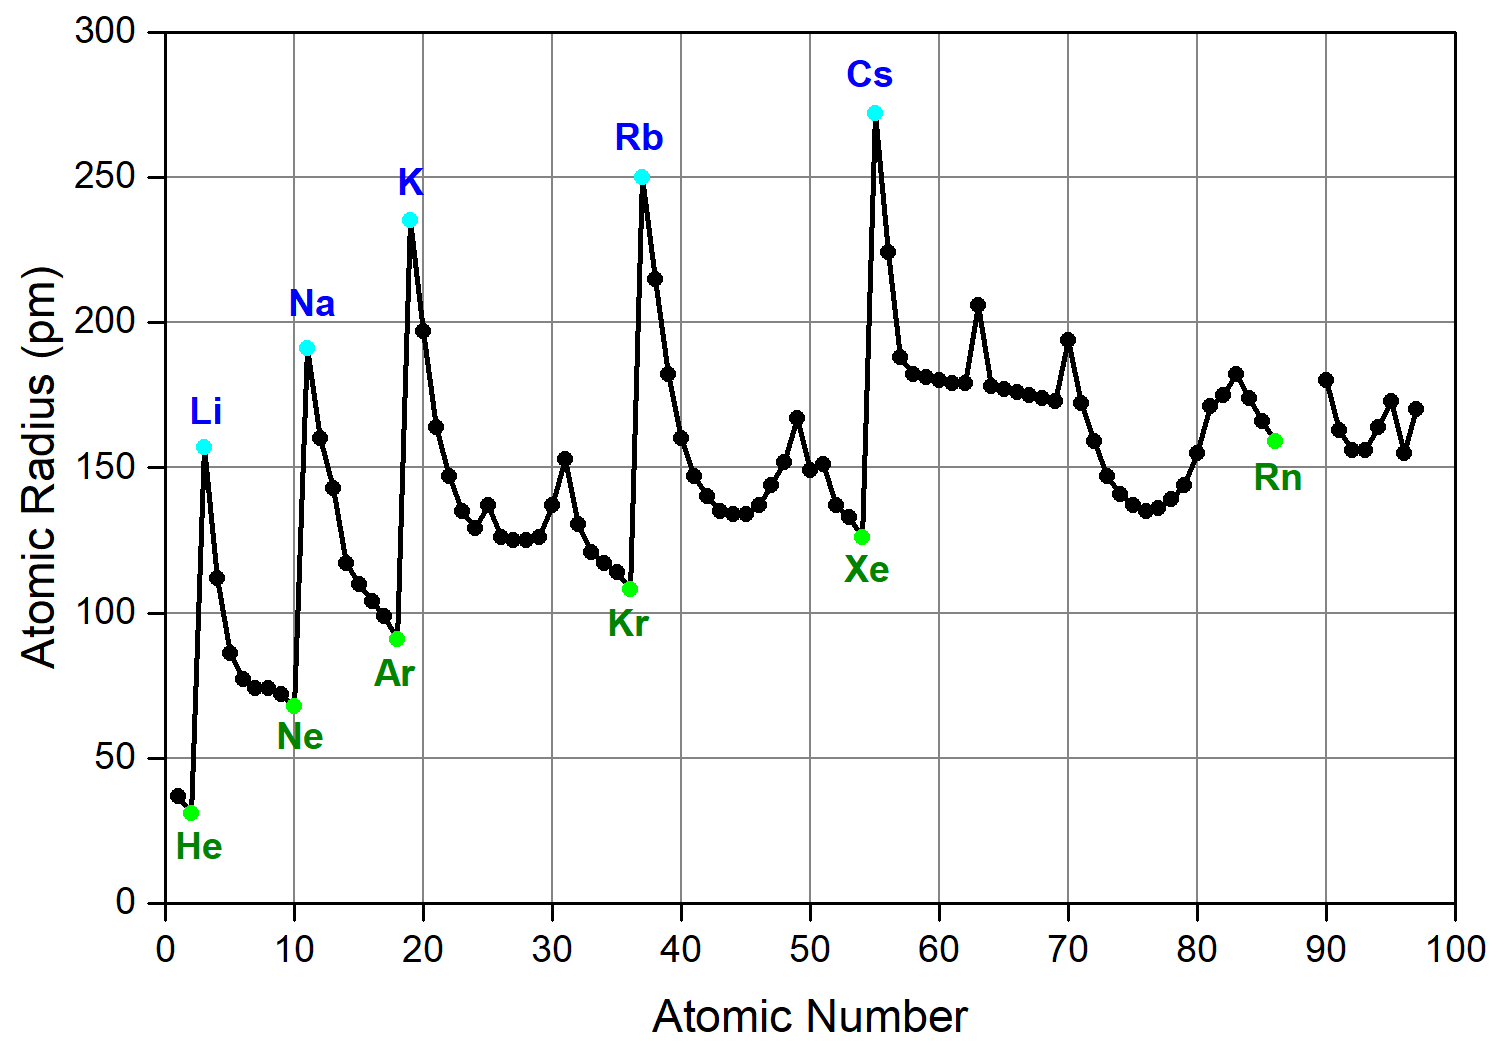
\includegraphics[width=0.45\textwidth]{atom-rad.png}
	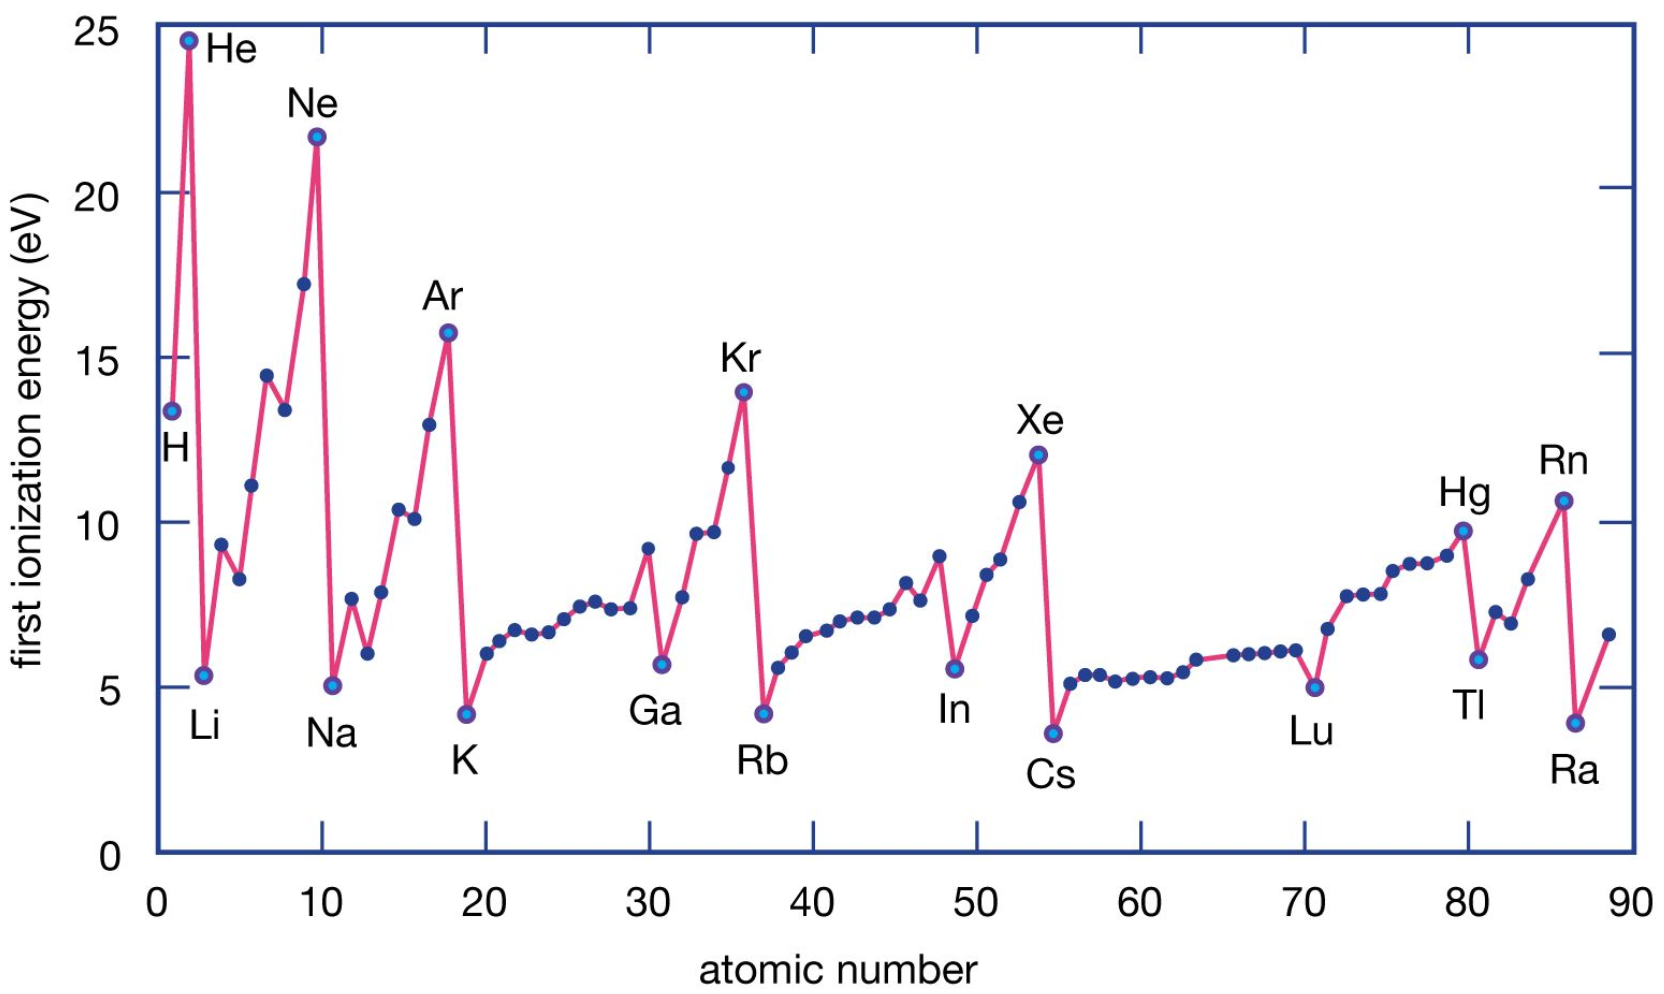
\includegraphics[width=0.52\textwidth]{atomic-ion-en.png}
	\caption{Atomic radius and ionization energy as functions of atomic mass number.}
	\label{atom-prop}
\end{figure}

\subsection{Evidenze sperimentali}

La semplicità del modello atomico a shell non è così immediata da traslare alla fisica nucleare: infatti, mentre gli elettroni nell'atomo sono soggette al campo coulombiano generato dal nucleo atomico, nel nucleo i nucleoni sono soggetti ad un campo che essi stessi generano, rendendo la trattazione analitica estremamente più complicata; inoltre, i nucleoni hanno un raggio relativamente grande rispetto al raggio del nucleo, a differenza degli elettroni che possono essere approssimati come point particles all'interno dell'atomo: ciò rende il concetto di orbite spaziali ben definite difficile da applicare al nucleo, dove il moto dei nucleoni può essere disturbato da urti con altri nucleoni.\\
Nonostante ciò, ci sono varie evidenze sperimentali che suggeriscono l'esistenza di shell nucleari.\\
Innanzitutto, se si plotta la binding energy per nucleone (Fig. \ref{magic-bind-en}), si notano delle consistenti deviazioni dalla formula di Weizsäcker per il liquid drop model in corrispodenza di precisi valori (uguali) di $ N $ e $ Z $, detti magic numbers: 2, 8, 20, 28, 50, 82, 126. Ciò significa che i nuclidi con determinati numeri di neutroni e/o protoni sono più legati, e dunque più stabili, dei nuclidi ad essi adiacenti. Per completezza, si ricordi che il liquid drop model non si applica per $ A < 20 $, poiché tali nuclidi presentano una struttura nucleare più complessa.

\begin{figure}[!t]
	\centering
	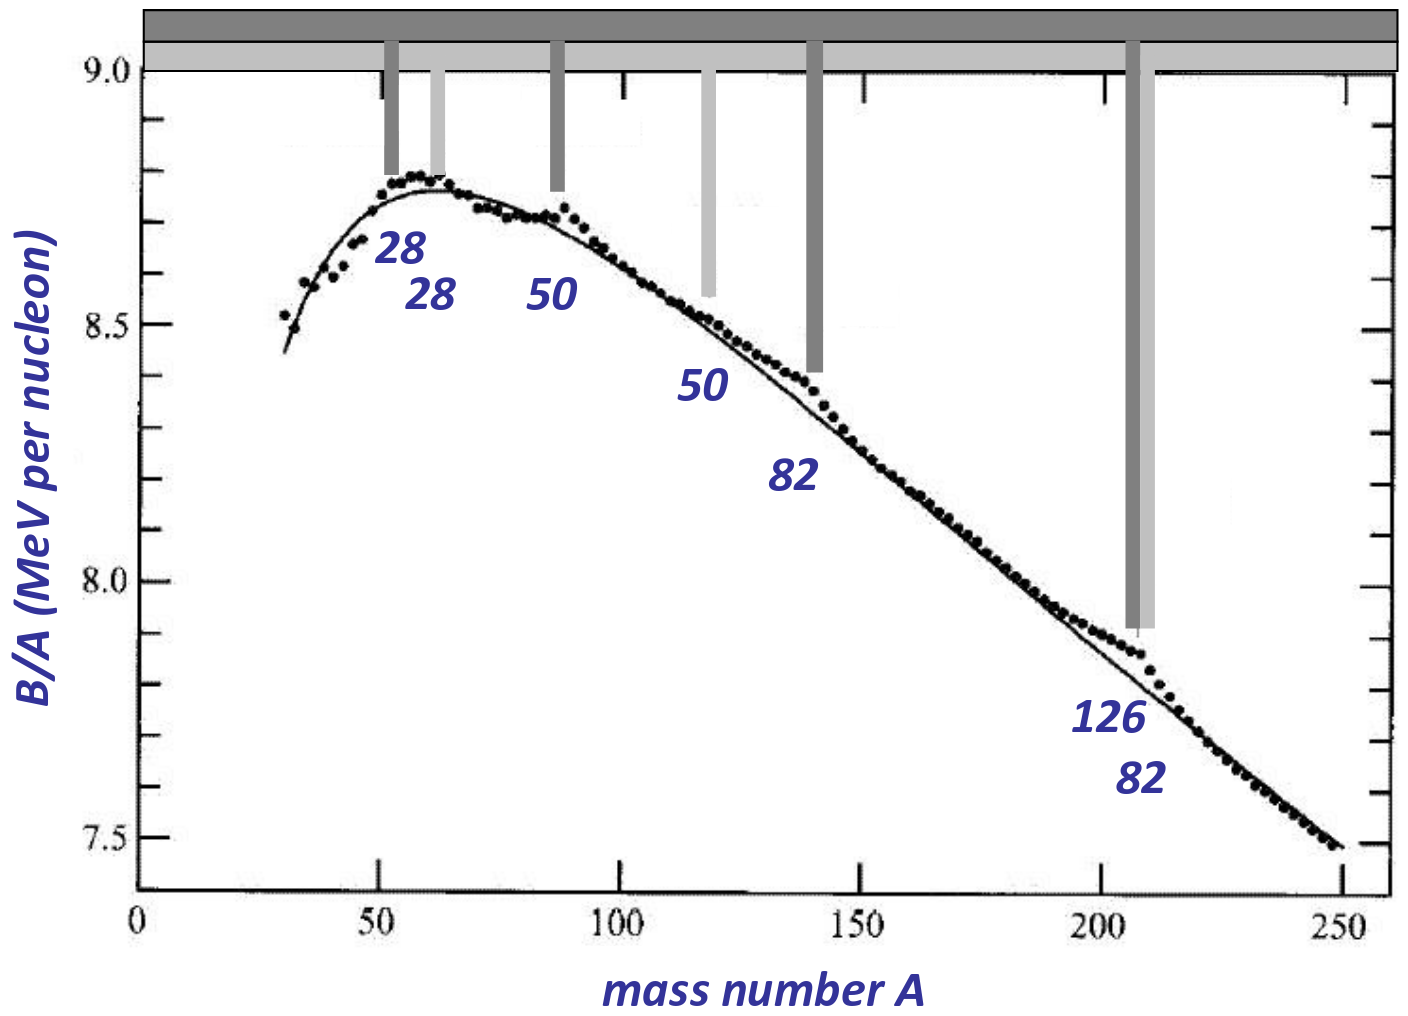
\includegraphics[width=0.60\textwidth]{magic-bind-en.png}
	\caption{Binding energy per nucleon, with $ N $ (dark grey) and $ Z $ (light grey) highlighted.}
	\label{magic-bind-en}
\end{figure}

\begin{figure}[!ht]
	\centering
	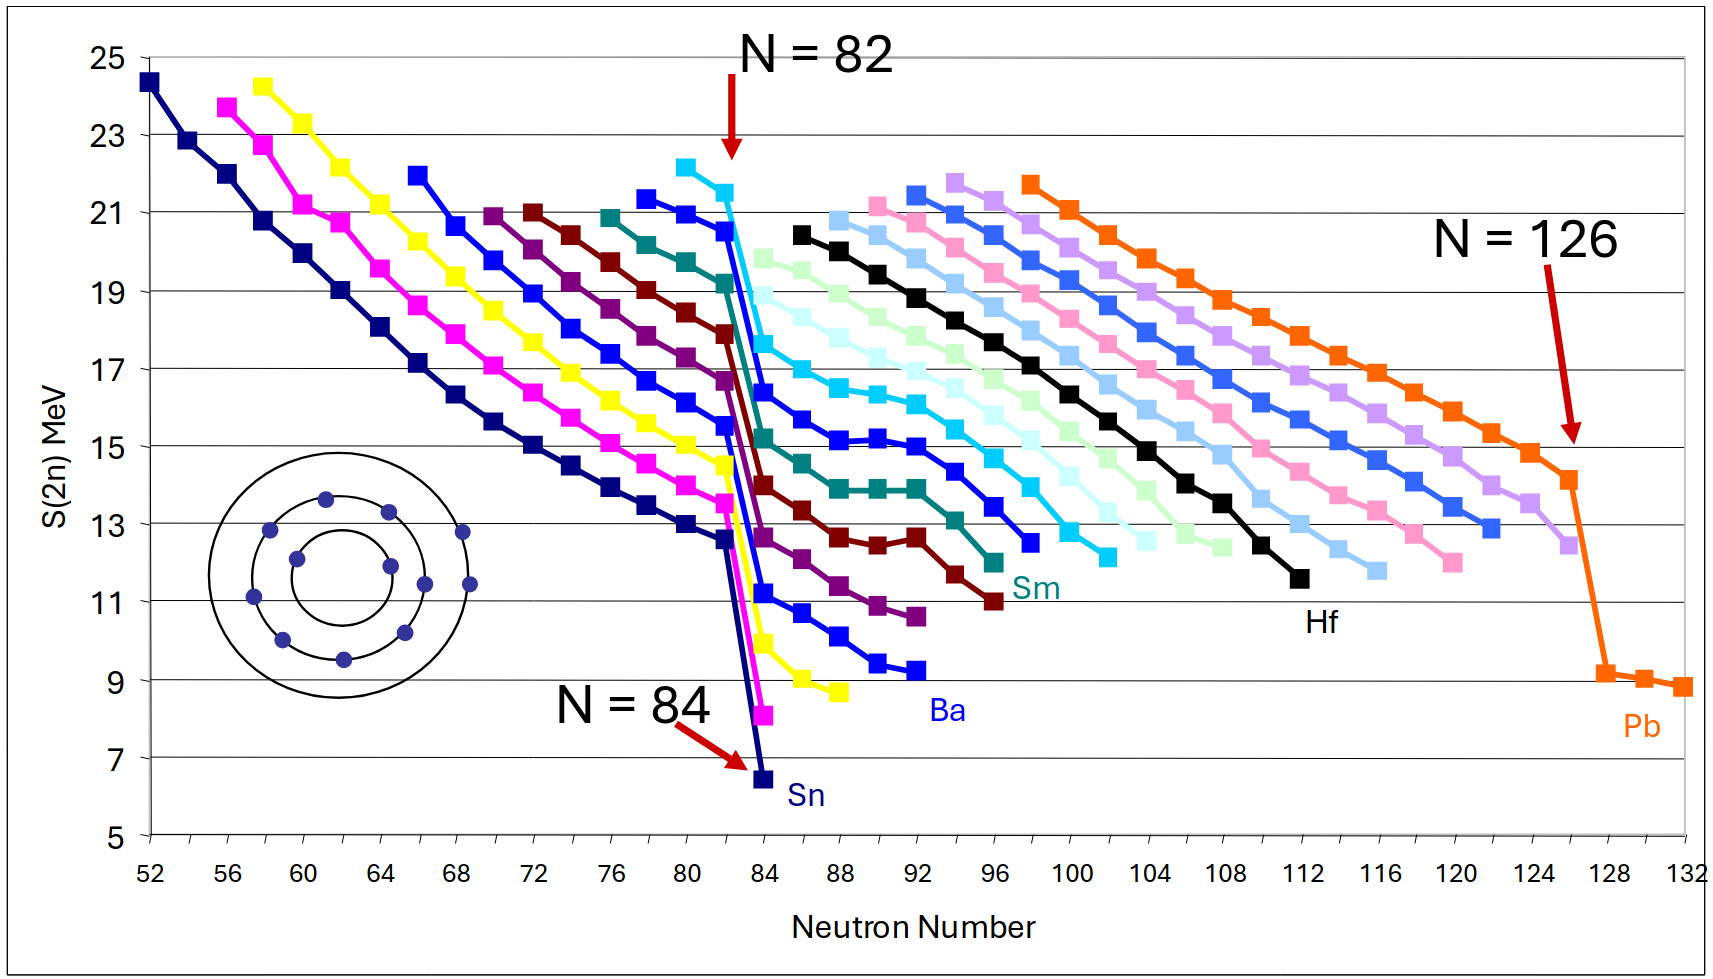
\includegraphics[width=0.60\textwidth]{2-n-b-e.png}
	\caption{2-neutron binding energy as a function of $ N $ for various isotopic chains.}
	\label{2-n-b-e}
\end{figure}

\begin{figure}[!t]
	\centering
	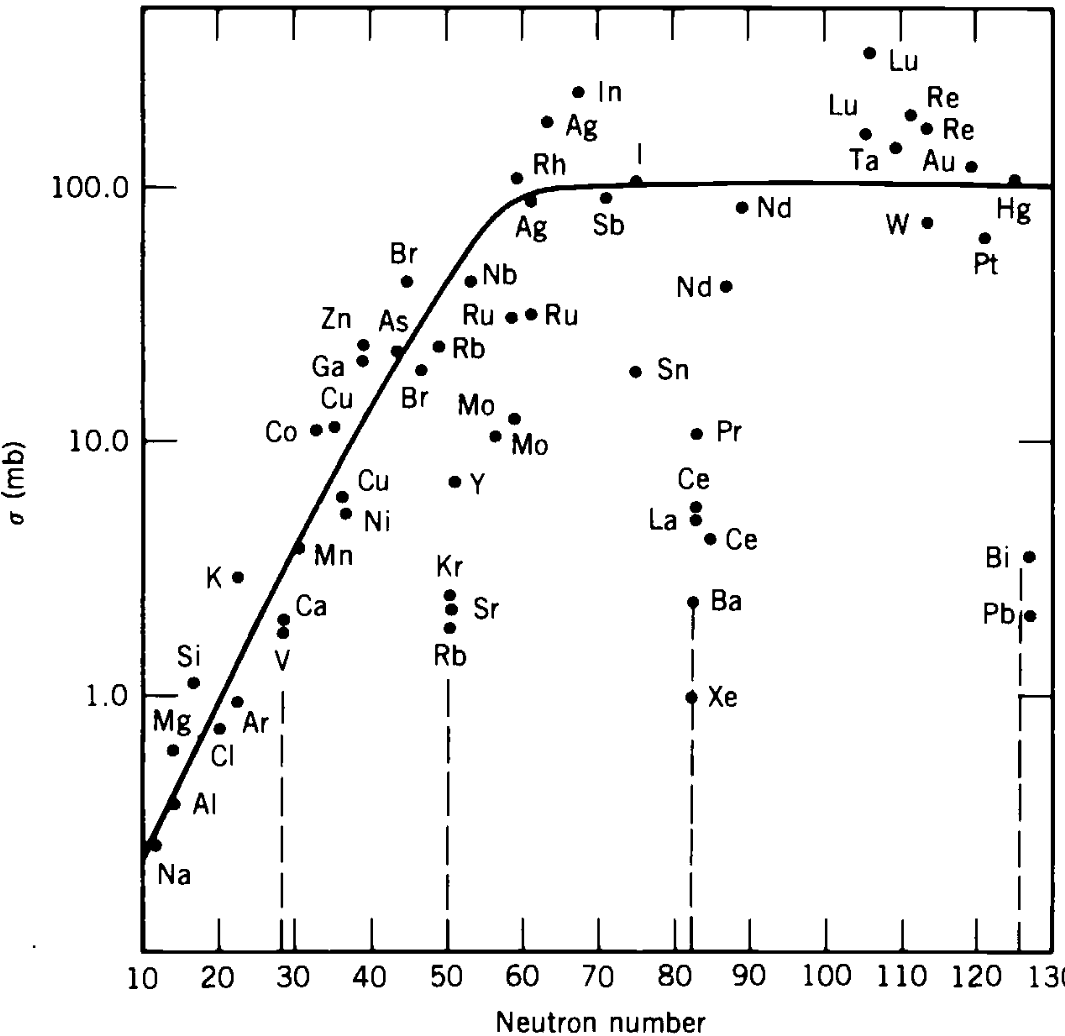
\includegraphics[width=0.60\textwidth]{magic-n-cap.png}
	\caption{$ n $-capture cross-section ad a funzion of.}
	\label{n-cap-cr}
\end{figure}

Gli stessi magic numbers si notano studiando la cosiddetta \textit{2-neutron binding energy}, ovvero la quantità $ S_{2n}(N,Z) \equiv B(N,Z) - B(N-2,Z) $, come si può vedere in Fig. \ref{2-n-b-e}: ciò può essere interpretato come una maggiore stabilità data dal completamento di shell neutroniche.\\
Anche l'abbondanza di isotopi stabili nel sistema solare mostra dei picchi in corrispondenza dei magic numbers, evidenziando la particolare stabilità dei nuclidi con shell closures.\\
Inoltre, la cross-section per la cattura neutronica subisce delle riduzioni di un paio di ordini di grandezza in corrispondenza dei magic numbers (Fig. \ref{n-cap-cr}: ciò è sia conseguenza diretta delle shell closures, sia conseguenza della riduzione del raggio nucleare determinato dalle suddette (dato che $ \sigma \sim \pi R^2 $).
Infine, per nuclei vicini ai magic numbers si osservano degli stati eccitati relativamente long-lived ($ \tau > 10^{-6}\,\text{s} $) detti \textit{isomeri}: i magic numbers determinano delle cosiddette $ \virgolette{islands of isomerism} $.\\
Si deve aggiungere poi che il liquid drop model non consente una descrizione di vari proprietà nucleari come lo spin, la parità, i momenti magnetici etc. Inoltre, esso non predice la densità nucleare e tutti i suoi coefficienti sono puramente empirici.

\subsection{Modello a particelle indipendenti}

Il primo modello a shell in grado di riprodurre i magic numbers e le proprietà dei magic nuclei fu formulato nel 1949 da Mayer e Jensen (entrambi Nobel nel 1963).\\
Il cosiddetto extreme single-particle shell model, detto anche shell model a particelle indipendenti, ha come assunzione di base che i nucleoni possano muoversi nel nucleo per la maggior parte del tempo senza interagire con altri nucleoni: ciò equivale a dire che il libero cammino medio di un nucleone è maggiore delle dimensioni del nucleo. Ovviamente questa è solo una semplificazione, dato che l'interazione tra nucleoni ha effetti importanti.\\
Rispetto allo shell model atomico, quello nucleare deve tener conto di alcune complicazioni: innanzitutto la forma del potenziale non è nota e, qualora lo si volesse assumere centrale, non ha avrebbe un centro definito poiché ciascun nucleone è sorgente del campo; inoltre, i nucleoni occupano il  nucleo in modo continuo, dunque non è ovvio come estendere il concetto di orbitale in questo contesto. Quest'ultima difficoltà è in parte ridotta dal principio d'esclusione di Pauli e dal modello a gas di Fermi\footnote{Un gas di Fermi è un modello ideale di un ensamble di molti fermioni non-interagenti in equilibrio termico, descritto dalla statistica di Fermi-Dirac.}: se il gas di nucleoni è fortemente degenere, ciascun nucleone è in uno stato quantistico e non scattera con un altro nucleone se non con un meccanismo di scambio, il che permette di impostare un'equazione del moto per il singolo nucleone (da qui il nome di modello a particelle indipendenti).\\
Per rendere l'equazione di Schrödinger risolvibile per un singolo nucleone, si applica l'\textit{approssimazione di campo medio}:
\begin{equation*}
	\hat{\mathcal{H}} = \sum_{j = 1}^{A} \frac{\hat{p}_j^2}{2m_j} + \sum_{j \neq k}^{A} \hat{V}_k(r_j) = \sum_{j = 1}^{A} \left[ \frac{\hat{p}_j^2}{2m_j} + \hat{V}(r_j) \right] + \sum_{j = 1}^{A} \underbrace{\left[ \sum_{k \neq j}^{A} \hat{V}_k(r_j) - \hat{V}(r_j) \right]}_{0}
\end{equation*}
dove l'approssimazione consiste nell'ultima semplificazione. Ciò permette di sostituire il termine d'interazione (che è a 2 corpi solo in prima approssimazione) con un potenziale centrale medio, ignorando l'interazione residua. Dato che il potenziale ha simmetria sferica, è possibile separare la funzione d'onda come:
\begin{equation}
	\psi(\ve{r}) = \frac{u_{\ell}}{r} Y_{\ell,m}(\theta,\phi) X_s
	\label{eq:5.3}
\end{equation}
recuperando così gli ususali numeri quantici. Rimane da determinare il potenziale; i tre potenziali usuali sono quello coulombiano, la buca di potenziale e quello armonico: il potenziale coulombiano non è adatto poiché l'interazione nucleare è a breve raggio e poiché non può riprodurre la saturazione delle forze nucleari; la buca di potenziale non è realistica poiché non può riprodurre l'energia cinetica e potenziale dei nucleoni; il potenziale armonico non va a 0 all'infinito, dunque non potrebbe descrivere la fuoriuscita di nucleoni dal nucleo, cosa che avviene se ad esempio viene aggiunto un nucleone ad un nuclide debolmente legato. Il potenziale che meglio rappresenta l'interazione nucleare è il \textit{potenziale di Woods-Saxon}:
\begin{equation}
	V_{\text{WS}}(r) = \frac{-V_0}{1 + e^{(r - R_0) / a}}
	\label{eq:5.4}
\end{equation}
dove $ V_0 \approx 50\mev $ (verso le driplines varia drasticamente), $ R_0 \approx 1.25\fm \cdot A^{1/3} $ è il raggio nucleare medio e $ a \approx 0.524\fm $ è la skin thickness del nucleo (distanza in cui $ V(r) $ passa da $ 0.9 V_0 $ a $ 0.1 V_0 $); esso è plottato in Fig. \ref{woods-saxon}.

\begin{figure}[!b]
	\centering
	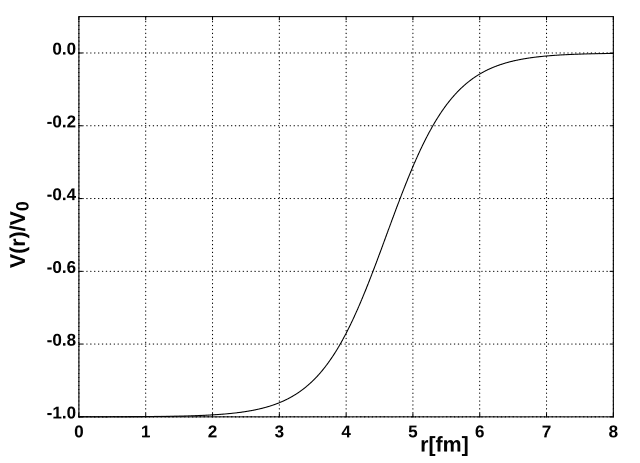
\includegraphics[width=0.70\textwidth]{woods-saxon.png}
	\caption{Woods-Saxon potential.}
	\label{woods-saxon}
\end{figure}

Il potenziale di Woods-Saxon prevede sia gli stati legati, con energia negativa, sia gli stati del continuo, con energia positiva. Gli stati sono giustamente quantizzati con tre numeri quantici: quello principale $ n $, quello angolare orbitale $ \ell $ e quello angolare totale $ j $ (relativo a $ \ve{J} = \ve{L} + \ve{S} $). Gli orbitali nucleari vengono quindi identificati come $ n\ell_j $, dove $ \ell $ è indicato con una lettera: $ s $ per $ \ell = 0 $, $ p $ per $ \ell = 1 $, $ d $ per $ \ell = 2 $, $ f $ per $ \ell = 3 $ e poi in ordine alfabetico.\\
Come si può vedere in Fig. \ref{ws-sp}, il solo potenziale di Woods-Saxon predice correttamente soltanto i primi tre magic numbers. È quindi necessario modificare tale potenziale con un termine di nuovo mutuato dalla fisica atomica: un termine d'interazione spin-orbita. Nel caso atomico, l'interazione spin-orbita avviene poiché il momento magnetico dell'elettrone interagisce col campo magnetico generato dal suo moto attorno al nucleo; nel caso nucleare, essa non deriva dall'interazione elettromagnetica ma dalla natura spin-dependent dell'interazione tra nucleoni.\\
Ricordando l'Eq. \ref{eq:4.20}, si può scrivere il \textit{potenziale d'interazione spin-orbita} come:
\begin{equation}
	V_{\ell,s}(r) \ve{L}\cdot\ve{S} = - \lambda \frac{1}{r} \frac{dV_{\text{WS}}}{dr} \ve{L}\cdot\ve{S}
	\label{eq:5.5}
\end{equation}
dove $ \lambda > 0 $ non ha particolare interesse fisico. Questo termine deriva dalla descrizione relativistica di un singolo nucleone nel nucleo ed è particolarmente importante sulla superficie nucleare (quando $ V_{\text{WS}}(r) $ varia maggiormente).

\begin{figure}[!b]
	\centering
	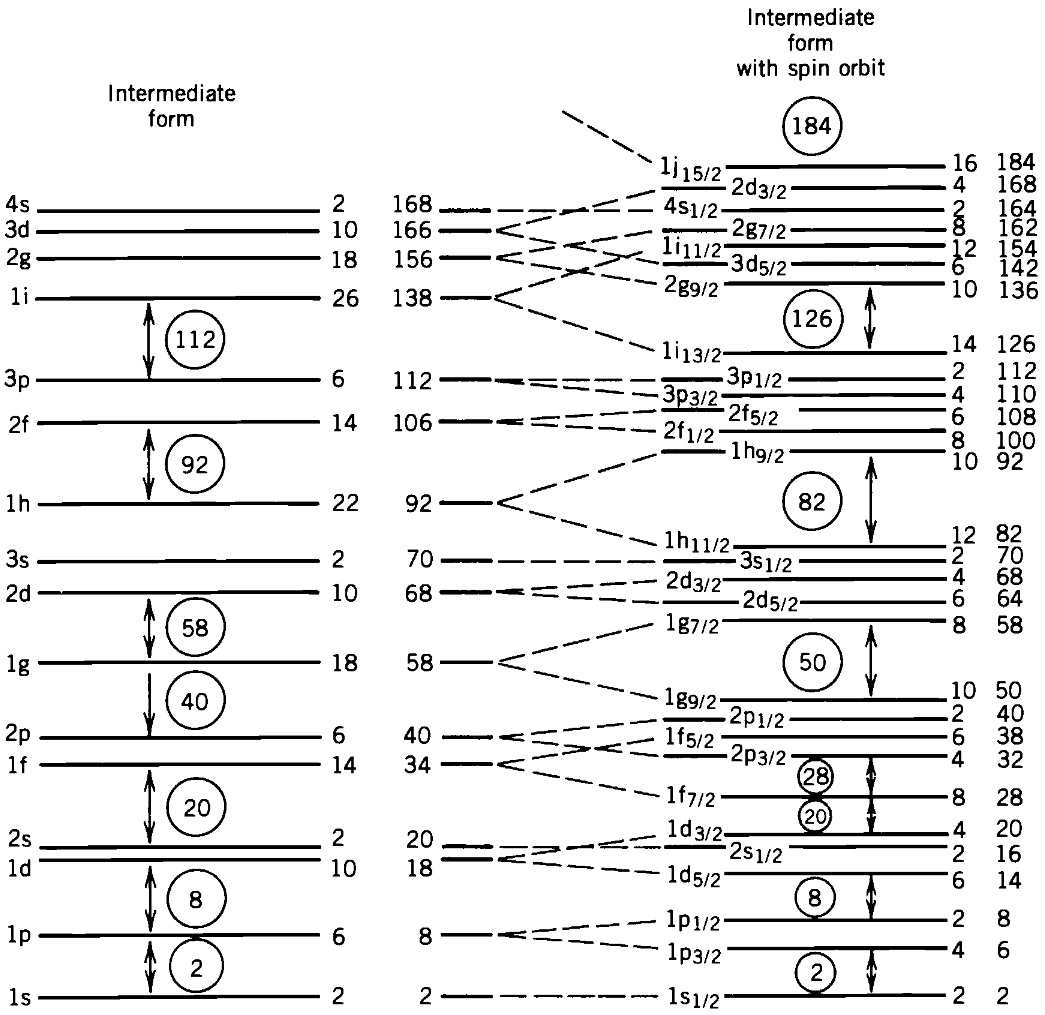
\includegraphics[width=0.60\textwidth]{ws-spectrum.png}
	\caption{Energy levels for the Woods-Saxon potential, without and with spin-orbit interaction.}
	\label{ws-sp}
\end{figure}

Si può vedere come l'aggiunta di questo termine splitti gli orbitali in modo da ottenere i corretti magic numbers. Ricordando che un nucleone ha $ s = \frac{1}{2} $, si vede che i possibili valori per $ j $ sono $ j = \ell + \frac{1}{2} $ e $ j = \ell - \frac{1}{2} $; inoltre, si può lavorare sul termine $ \ve{L}\cdot\ve{S} $:
\begin{equation*}
	\braket{\ve{L}\cdot\ve{S}} = \frac{1}{2} \braket{\ve{J}^2 - \ve{L}^2 - \ve{S}^2} = \frac{\hbar^2}{2} \left[ j (j + 1) - \ell (\ell + 1) - s (s + 1) \right]
\end{equation*}
A questo punto, si deve considerare che i due possibili valori di $ j $ per ogni $ \ell $ portano ad uno split degli orbitali considerati: ad esempio, un orbitale $ 1f $ (con $ \ell = 3 $) viene splittato in $ 1f_{5/2} $ e $ 1f_{7/2} $. Ciascun orbitale così ottenuto ha degenerazione $ 2j + 1 $ determinata da $ m_j $ (con l'interazione spin-orbita, $ m_{\ell} $ ed $ m_s $ non vanno più bene come numeri quantici poiché non sono ben definiti): in questo modo si ottiene comunque la corretta degenerazione totale, poiché $ 2(\ell + \frac{1}{2}) + 1 + 2(\ell - \frac{1}{2}) + 1 = 2(2\ell + 1) $, solo che viene redistribuita asimmetricamente tra due orbitali.\\
Questo splitting porta ad uno splitting anche energetico proporzionale ad $ \ell $, poiché:
\begin{equation}
	\braket{\ve{L}\cdot\ve{S}}_{j = \ell + \frac{1}{2}} - \braket{\ve{L}\cdot\ve{S}}_{j = \ell - \frac{1}{2}} = \frac{\hbar^2}{2} (2\ell + 1)
	\label{eq:5.6}
\end{equation}
Dato che $ V_{\ell,s}(r) < 0 $ (dall'Eq. \ref{eq:5.5}), l'orbitale con $ j $ maggiore ha un'energia più bassa: come si vede in Fig. \ref{ws-sp}, ciò permette di ottenere i corretti magic numbers ed anche di predirne uno nuovo ancora mai osservato: 184.\\
Un'importante conseguenza di questo splitting è che orbitali con diverso $ n $ ed $ \ell $ vengono scambiati di posto nella ladder degli stati: di conseguenza, dato che la parità di un orbitale è $ \pi = (-1)^{\ell} $, orbitali di parità diversa vengono mescolati nella ladder; inoltre, dato che l'interazione forte preserva la parità, orbitali di parità diversa sono ben distinti tra loro e possono essere considerati degli stati puri.

\subsubsection{Nucleoni di valenza}

Il modello a shell, nella sua versione più semplice, ascrive tutte le proprietà di un nuclide dispari (ovvero con $ A $ dispari) al singolo nucleone spaiato nella shell più esterna: se esso si trova nell'orbitale $ n\ell_j $, il ground state del nuclide avrà spin $ j $ e parità $ (-1)^{\ell} $.\\
Nonostante l'estrema semplicità, questo modello predice correttamente il $ J^{\pi} $ di praticamente tutti i nuclidi dispari nel range di masse in cui il modello a shell è valido (ossia $ A < 150 $ e $ 190 < A < 220 $).
Un calcolo più preciso deve ovviamente tener conto almeno di tutti i nucleoni sulla shell di valenza: in tal caso, ciascuno stato eccitato può essere ottenuto mediante varie eccitazioni di nucleoni diversi (sovrapposizione di stati), dette particle-hole eccitations: passando da una shell di energia minore ad una di energie maggiore, il nucleone lascia un buco nella shell minore e questo processo richiede una notevole energia, specialmente se nei pressi degli shell gaps. Anche in questo caso, si ha un buon accordo per nuclidi dispari, specialmente per quelli esprimibili come un doubly magic nuclei + uno o più (pochi) nucleoni (es.: elio, ossigeno, calcio, etc.).\\
In generale (quindi anche per nuclidi pari), ogni orbitale completamente pieno di nucleoni non contribuisce allo spin nucleare, dato che essi si accoppiano in coppie di nucleoni identici con spin opposti (configurazione energeticamente più favorevole).

\subsubsection{Momento magnetico}

Dall'Eq. \ref{eq:4.14}, considerando un $ g_{\ell} $ generico (e non il caso specifico $ g_{\ell} = \frac{1}{2} $), si ha:
\begin{equation}
	g_j = \frac{1}{2} (g_{\ell} + g_s) + \frac{1}{2} \frac{\ell (\ell + 1) - s (s + 1)}{j (j + 1)} (g_{\ell} - g_s)
	\label{eq:5.7}
\end{equation}
I momenti magnetici nucleari possono dunque essere calcolati come:
\begin{equation}
	\braket{\mu} =
	\begin{cases}
		\left[ g_{\ell} (j - \frac{1}{2}) + \frac{1}{2} g_s \right] \mu_N & j = \ell + \frac{1}{2} \\
		\frac{j}{j + 1} \left[ g_{\ell} (j + \frac{3}{2}) - \frac{1}{2} g_s \right] \mu_N & j = \ell - \frac{1}{2}
	\end{cases}
	\label{eq:5.8}
\end{equation}
Queste sono le cosiddette \textit{linee di Schmidt} e, se moltiplicate per un fattore di scala di circa $ 0.60 $, riproducono il trend seguito dai dati sperimentali, come si può vedere in Fig. \ref{schmidt}.

\begin{figure}[!t]
	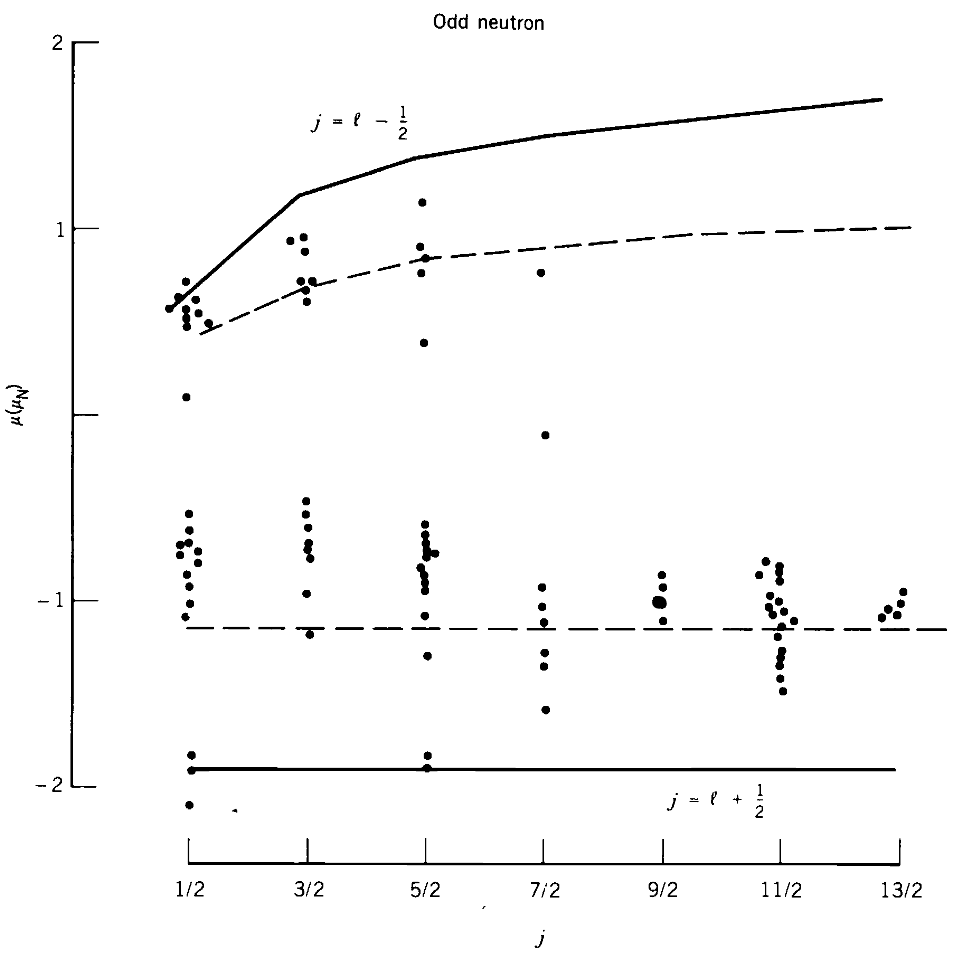
\includegraphics[width=0.60\textwidth]{schmidt-1.png}
	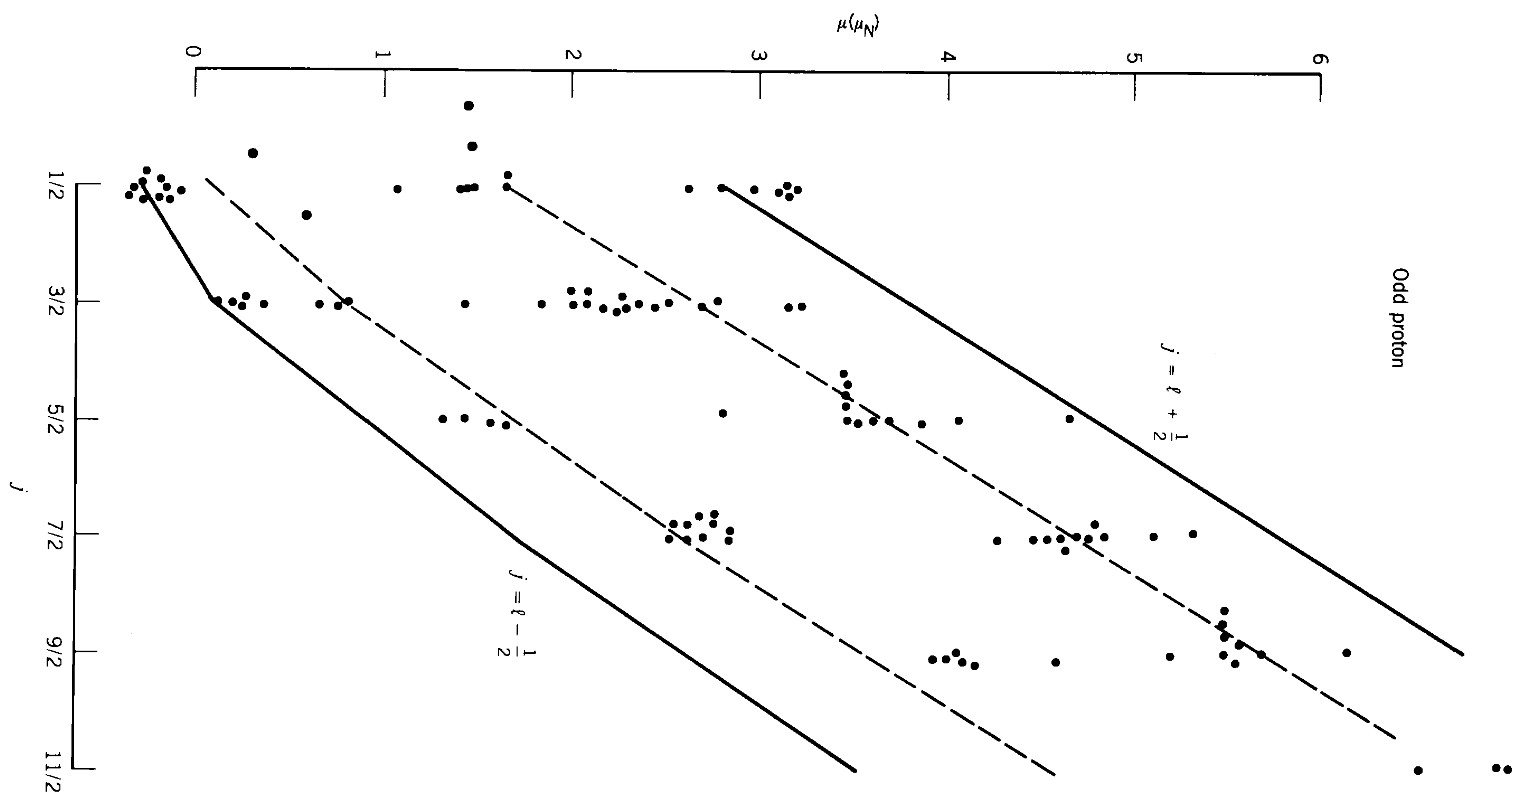
\includegraphics[angle=90,width=0.35\textwidth]{schmidt-2.png}
	\caption{Schmidt lines.}
	\label{schmidt}
\end{figure}

Lo scatter dei dati rispetto alle linee di Schmidt indica che il calcolo del momento magnetico considerando i nucleoni come indipendenti è una semplificazione eccessiva; per un calcolo più preciso, si dovrebbero considerare degli effetti non-banali come l'influenza reciproca dei nucleoni, il fatto che lo spin pairing non sia perfetto, le nubi mesoniche che circondano i nucleoni (che contengono pioni $ \pi^{\pm} $ carichi) e la non sfericità dei nuclei.

\subsubsection{Interazione residua}

Per dare una descrizione unificata di tutti i nuclidi, è necessario aggiungere allo shell model la descrizione dell'interazione residua che viene ignorata nel modello. Ad esempio, per nuclei leggeri è necessario considerare interazioni nucleari a tre o più corpi, problemi difficoltosi da trattare in QCD.\\
Ad oggi, un modo computazionalmente efficiente di calcolare l'interazione residua è dividere il nuclide in un core composto dal più vicino doubly-magic nuclei ($ \ch{^4He} $, $ \ch{^{16}O} $, $ \ch{^{40}Ca} $, $ \ch{^{132}Sn} $ e $ \ch{^{208}Pb} $), il quale rimane freezato e non viene considerato nelle interazioni, e le rimanenti shell d'interazione. Dato che il numero di modi di distribuire $ k $ nucleoni su $ n $ orbitali è pari a $ \binom{n}{k} $, che aumenta fattorialmente all'aumentare dei nucleoni, per snellire ulteriormente il calcolo dal punto di vista computazionale si può ulterioremente restringere l'insieme dei nucleoni sui quali calcolare l'interazione residua alla sola shell di valenza.\\
Anche in questo caso ci sono però delle limitazioni, prime su tutti il considerare solo i nucleoni di valenza e l'ignorare completamente le eccitazioni del core.\\
I principali filoni di ricerca a livello computazionale riguardano da un lato la risoluzione numerica della many-body hamiltonian, dall'altro lo studio delle interazioni nucleari.

\section{Collective models}

Il modello a shell descrive molto bene i nuclidi nell'intorno dei magic numbers, per i quali vale l'approssimazione di campo medio. Quando però si considerano nuclei lontani da tali regioni, i dati sperimentali si discostano dalle previsioni del modello a shell: si osservano fenomeni non riconducibili ad eccitazioni individuali di nucleoni che suggeriscono un comportamento collettivo del sistema.

\subsection{Evidenze sperimentali}

La principale limitazione del modello a shell è l'assunzione che il nucleo sia sferico: ciò è approssimativamente vero solo per nuclei vicini ai doubly-magic nuclei, i quali hanno una doppia shell closure, ma in generale non è vero. La deformazione dei nuclidi lontani dai magic numbers è suggerita da varie evidenze sperimentali, come un grande momento di quadrupolo elettrico (discostamento dalla simmetria di carica), una bassa excitation energy ($ < 1\mev $) per il primo stato eccitato nei nuclei pari-pari (quasi sempre il $ 2^+ $) ed un rapporto costante $ E(4^+) / E(2^+) $ sempre per nuclei pari-pari.

\subsubsection{Momento di quadrupolo elettrico}

Ricordando la definizione in Eq. \ref{eq:4.16}, i momenti di multipolo elettrico forniscono una descrizione della distribuzione di carica (dunque dei protoni) nel nucleo.\\
Dato che i momenti dispari devono essere nulli per la conservazione della parità e che $ K_0 = Ze $ non è altro che la carica totale, il primo parametro utile a verificare la deviazione della distribuzione di carica da una forma sferica è il momento di quadrupolo elettrico $ K_2 \equiv Q $, definito in Eq. \ref{eq:4.17}: assumendo che le distribuzioni di protoni e neutroni non siano troppo diverse tra loro (vero nella valle di stabilità), si può prendere il momento di quadrupolo elettrico come un indicatore della deformazione del nucleo stesso.\\
Considerando un nucleo a forma di ellissoide con sezione circolare di raggio $ a $ sul piano $ xy $ e semiasse $ b $ sull'asse $ z $, si può definire un parametro di deformazione $ \beta $ in funzione del raggio medio $ \braket{R} = (ab^2)^{1/3} $ e della differenza dei semiassi $ \Delta R = b - a $:
\begin{equation}
	\beta = \frac{4}{3} \sqrt{\frac{\pi}{5}} \frac{\Delta R}{\braket{R}}
	\label{eq:5.9}
\end{equation}
In base al segno di $ \beta $, si può stabilire se il nucleo è sferico ($ \beta = 0 $), prolato (allungato lungo $ z $, $ \beta > 0 $) o oblato (schiacciato su $ xy $, $ \beta < 0 $). Il momento di quadrupolo elettrico è legato a $ \beta $ da:
\begin{equation}
	Q_0 = \frac{3}{\sqrt{5\pi}} Z \braket{R}^2 \beta (1 + 0.16 \beta)
	\label{eq:5.10}
\end{equation}
Si noti che $ Q_0 $ è il momento di quadrupolo intrinseco, ovvero misurato nel RF solidale al nuclide; il momento misurato in laboratorio $ Q $ è legato a $ Q_0 $ da una relazione che varia per i vari stati eccitati: per lo stato $ 2^+ $, si ha $ Q = - \frac{2}{7} Q_0 $.
Come si può vedere in Fig. \ref{quad-mom}, i nuclei vicini ai magic numbers sono praticamente sferici, mentre quelli lontani da essi sono deformati: in particolare, i nuclei delle terre rare sono stabilmente deformati. Inoltre, si nota una prevalenza di nuclei prolati rispetto a quelli oblati.

\begin{figure}[!t]
	\centering
	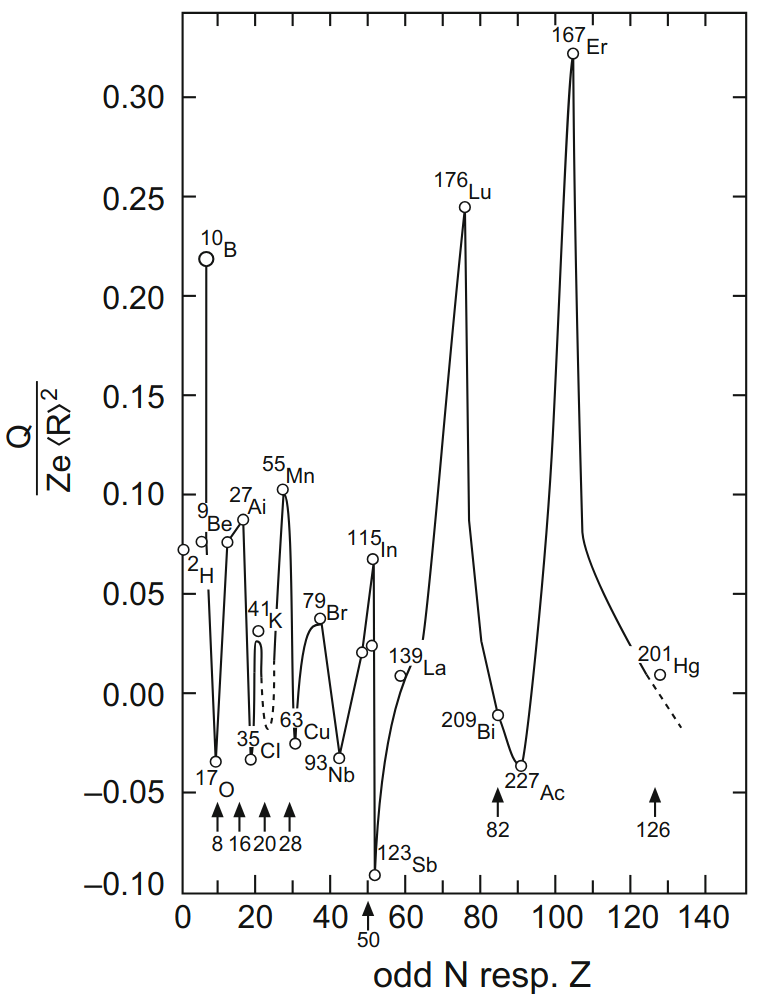
\includegraphics[width=0.60\textwidth]{quad-mom.png}
	\caption{Nuclear electric quadrupole moments for nuclei with odd nucleons.}
	\label{quad-mom}
\end{figure}

\subsubsection{Energia dello stato \texorpdfstring{$ 2^+ $}{TEXT}}

Mentre le eccitazioni dei nuclei dispari sono spiegate bene dal modello a shell, per i nuclei pari-pari il modello non funziona, in quanto in prima approssimazione tutti gli spin dei nucleoni si dovrebbero accoppiare a 0: con tale modello, dunque, è difficile spiegare i loro stati eccitati.\\
Per i nuclei pari-pari, il ground state è lo stato $ 0^+ $ ed il primo stato eccitato è lo stato $ 2^+ $: per spiegare questo stato col modello a shell, sarebbe necessario rompere una coppia di nucleoni appaiati ed eccitarli su livelli distinti, impiegando una notevole quantità di energia ($ \approx 2\mev $). Studiando le energie degli stati $ 2^+ $, però, si vede (Fig. \ref{2-p}) che tale soglia è raggiunta solo nei pressi delle shell closures, mentre normalmente si hanno energie al di sotto di $ 1.2\mev $ con un trend decrescente, fino ad arrivare a $ 100\kev $ per nuclidi pesanti; si nota inoltre che per $ 150 < A < 190 $ e $ A > 230 $ l'energia $ E(2^+) $ è praticamente costante.\\
Da queste osservazioni si conclude che, per realizzare il primo stato $ 2^+ $, questi nuclei assumano una configurazione intrinsecamente più conveniente a livello energetico rispetto alla rottura di una coppia nucleonica.

\begin{figure}[!t]
	\centering
	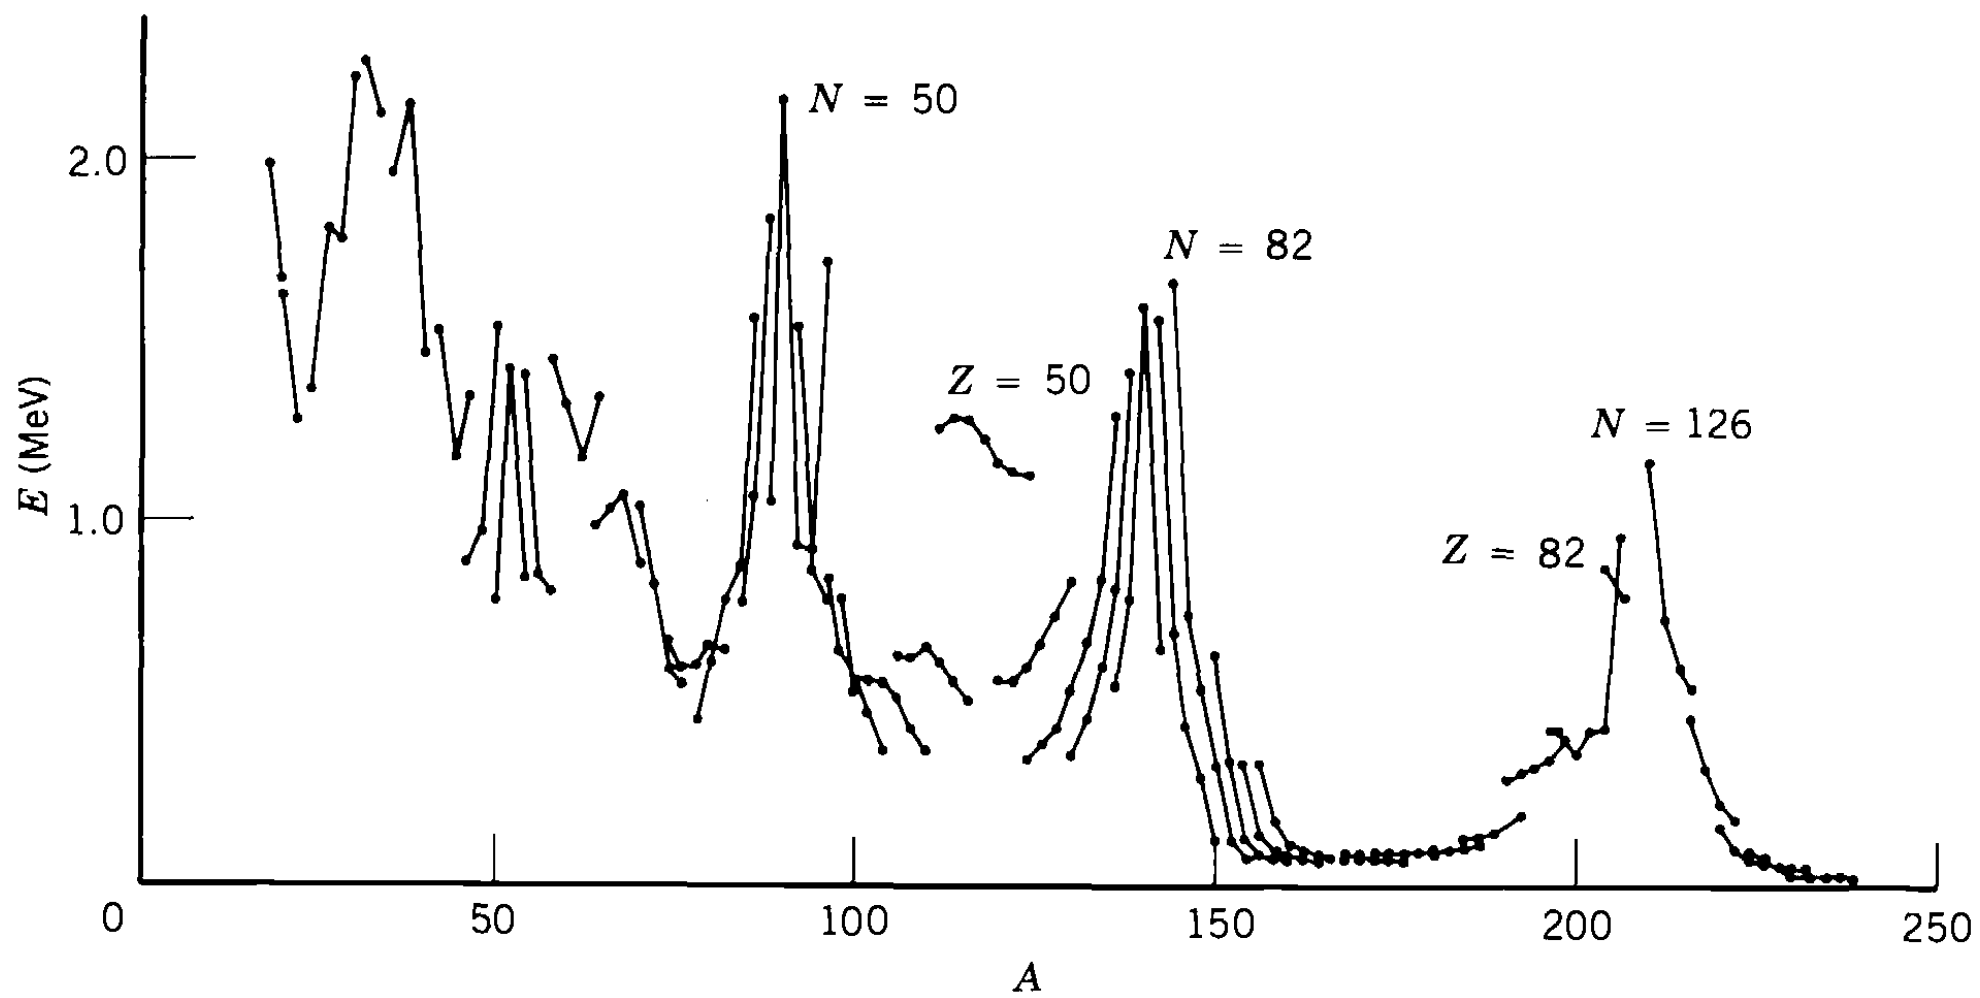
\includegraphics[width=0.70\textwidth]{2-p.png}
	\caption{Energies of lowest $ 2^+ $ states of even-even nuclei, with isotopic chains connected.}
	\label{2-p}
\end{figure}

\subsubsection{Andamento anomalo di \texorpdfstring{$ E(4^+) / E(2^+) $}{TEXT} e \texorpdfstring{$ Q(2^+) $}{TEXT}}

\begin{figure}[!b]
	\centering
	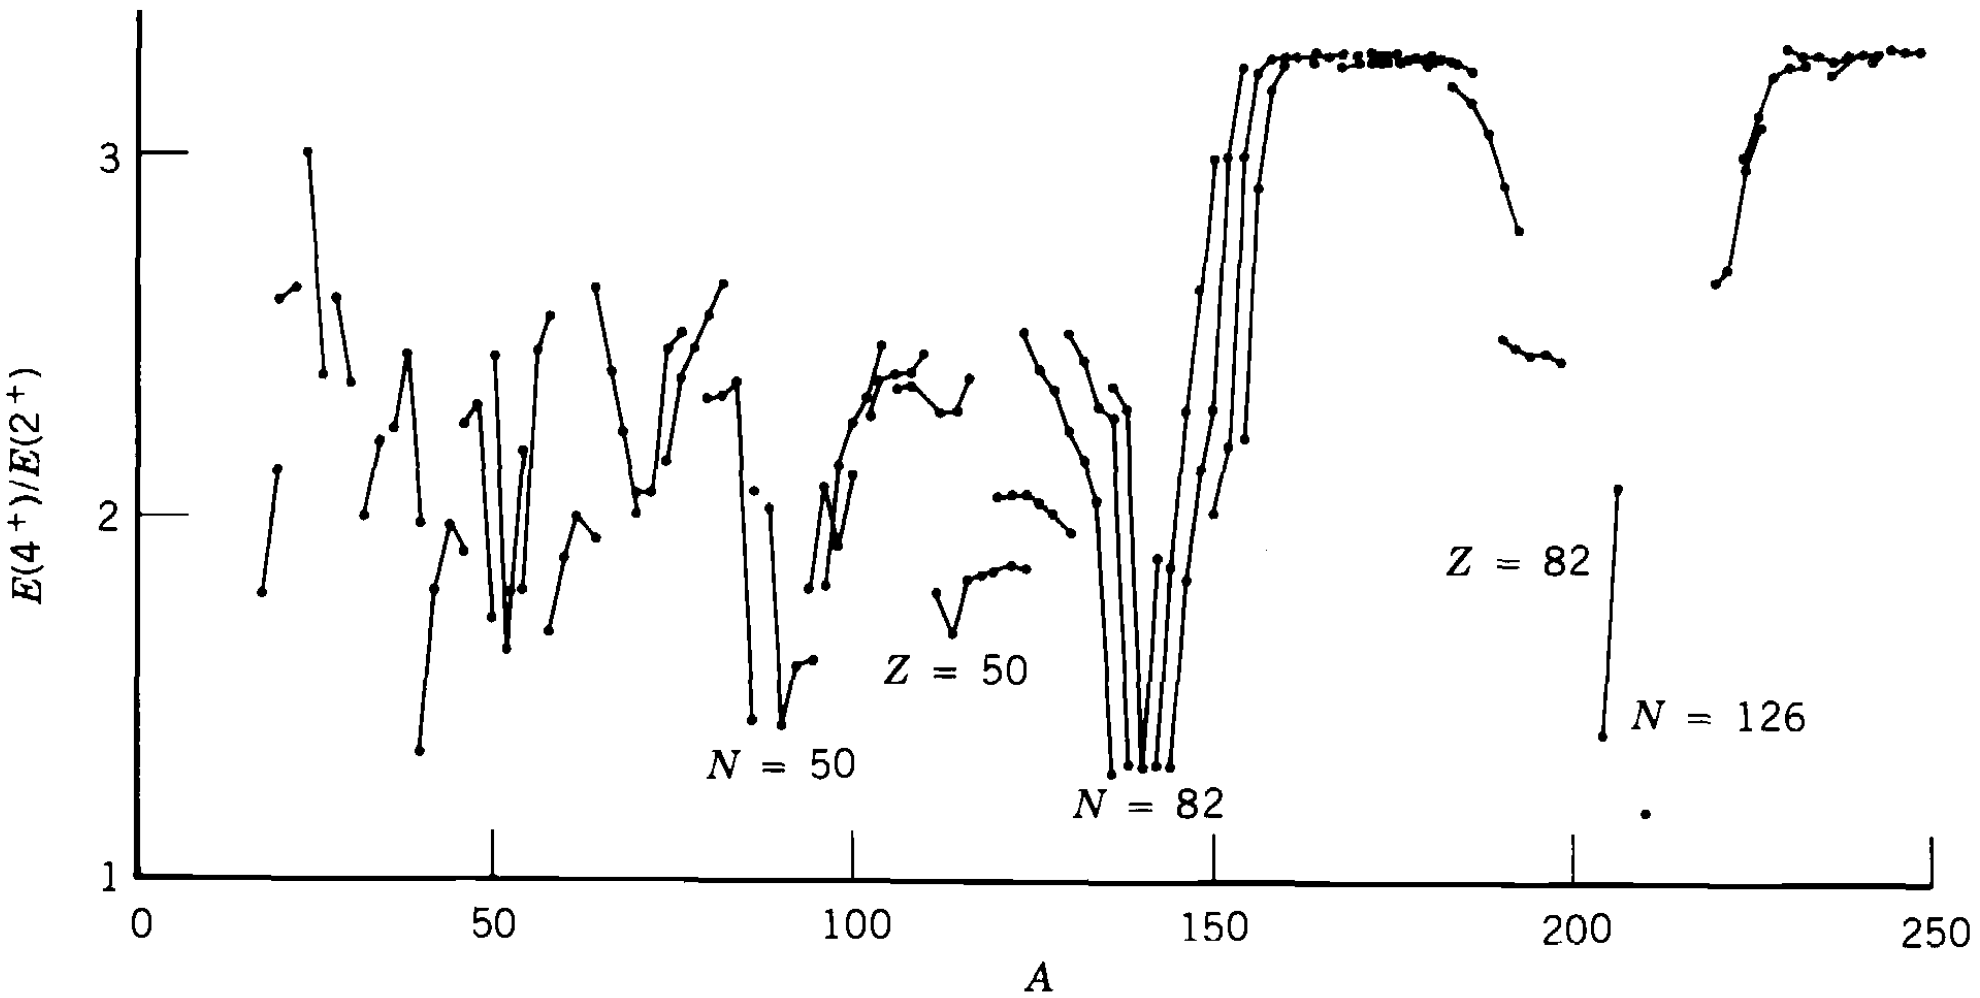
\includegraphics[width = 0.54 \textwidth]{4-p-2-p.png}
	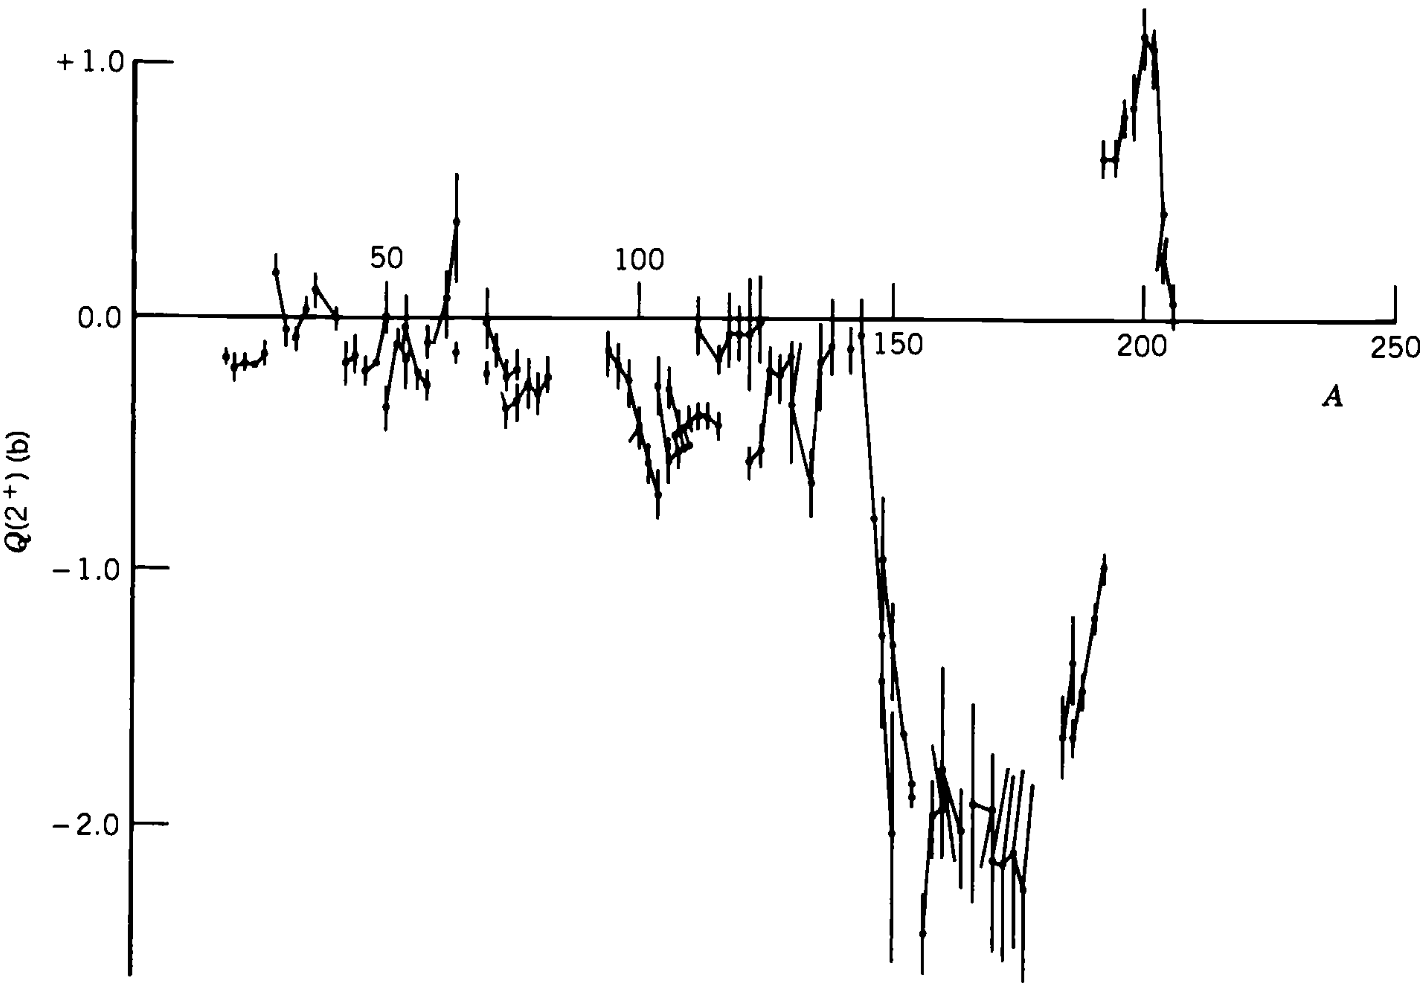
\includegraphics[width = 0.45 \textwidth]{q-2.png}
	\caption{$ E(4^+) / E(2^+) $ ratio and $ Q(2^+) $ for even-even nuclei.}
	\label{4-p-2-p}
\end{figure}

Studiando il rapporto delle energie per i primi stati eccitati $ 2^+ $ e $ 4^+ $ dei nuclei pari-pari (Fig. \ref{4-p-2-p}) si nota che per $ A < 150 $ c'è uno scatter attorno al valore 2, mentre per $ 150 < A < 190 $ e $ A > 230 $ il rapporto ha un valore costante pari a 3.3, indipendentemente dal nuclide considerato.\\
Un trend simile si evidenzia nello studio del momento di quadrupolo magnetico per lo stato $ 2^+ $ (Fig. \ref{4-p-2-p}): per $ A < 150 $ questo momento è circa nullo (a parte deformazioni lontane dalle shell closures), mentre si hanno importanti deviazioni per $ A > 150 $.

\subsubsection{Moti nucleari collettivi}

Tutte queste evidenze sperimentali suggeriscono due tipi diversi di moti nucleari collettivi: le vibrazioni collettive e le rotazioni collettive (vedere Fig. \ref{coll}). Questi moti collettivi avvengono assieme alle eccitazioni single particle del modello a shell e danno una spiegazione a stati che lo shell model non prevede.\\
Per nuclei con $ A < 150 $ si hanno principalmente delle vibrazioni attorno ad una forma sferica: la forma media nel tempo è comunque quella sferica, ma le eccitazioni causano delle vibrazioni collettive del sistema; la sequenza degli stati eccitati generati dalle vibrazioni collettive è energeticamente equispaziata e ha forma $ E_n = n \hbar \omega $.\\
Nuclei con $ A > 150 $ invece sono permanente deformati e hanno un moto rotatorio collettivo; le eccitazioni hanno energia $ E_{I} = \frac{\hbar^2}{2\mathfrak{I}} I (I + 1) $, con $ \mathfrak{I} $ il momento d'inerzia del nucleo e $ I $ il quantum number associato al momento angolare totale (sia neutroni che protoni), dunque sono progressivamente sempre più energeticamente separate.

\begin{figure}[!t]
	\centering
	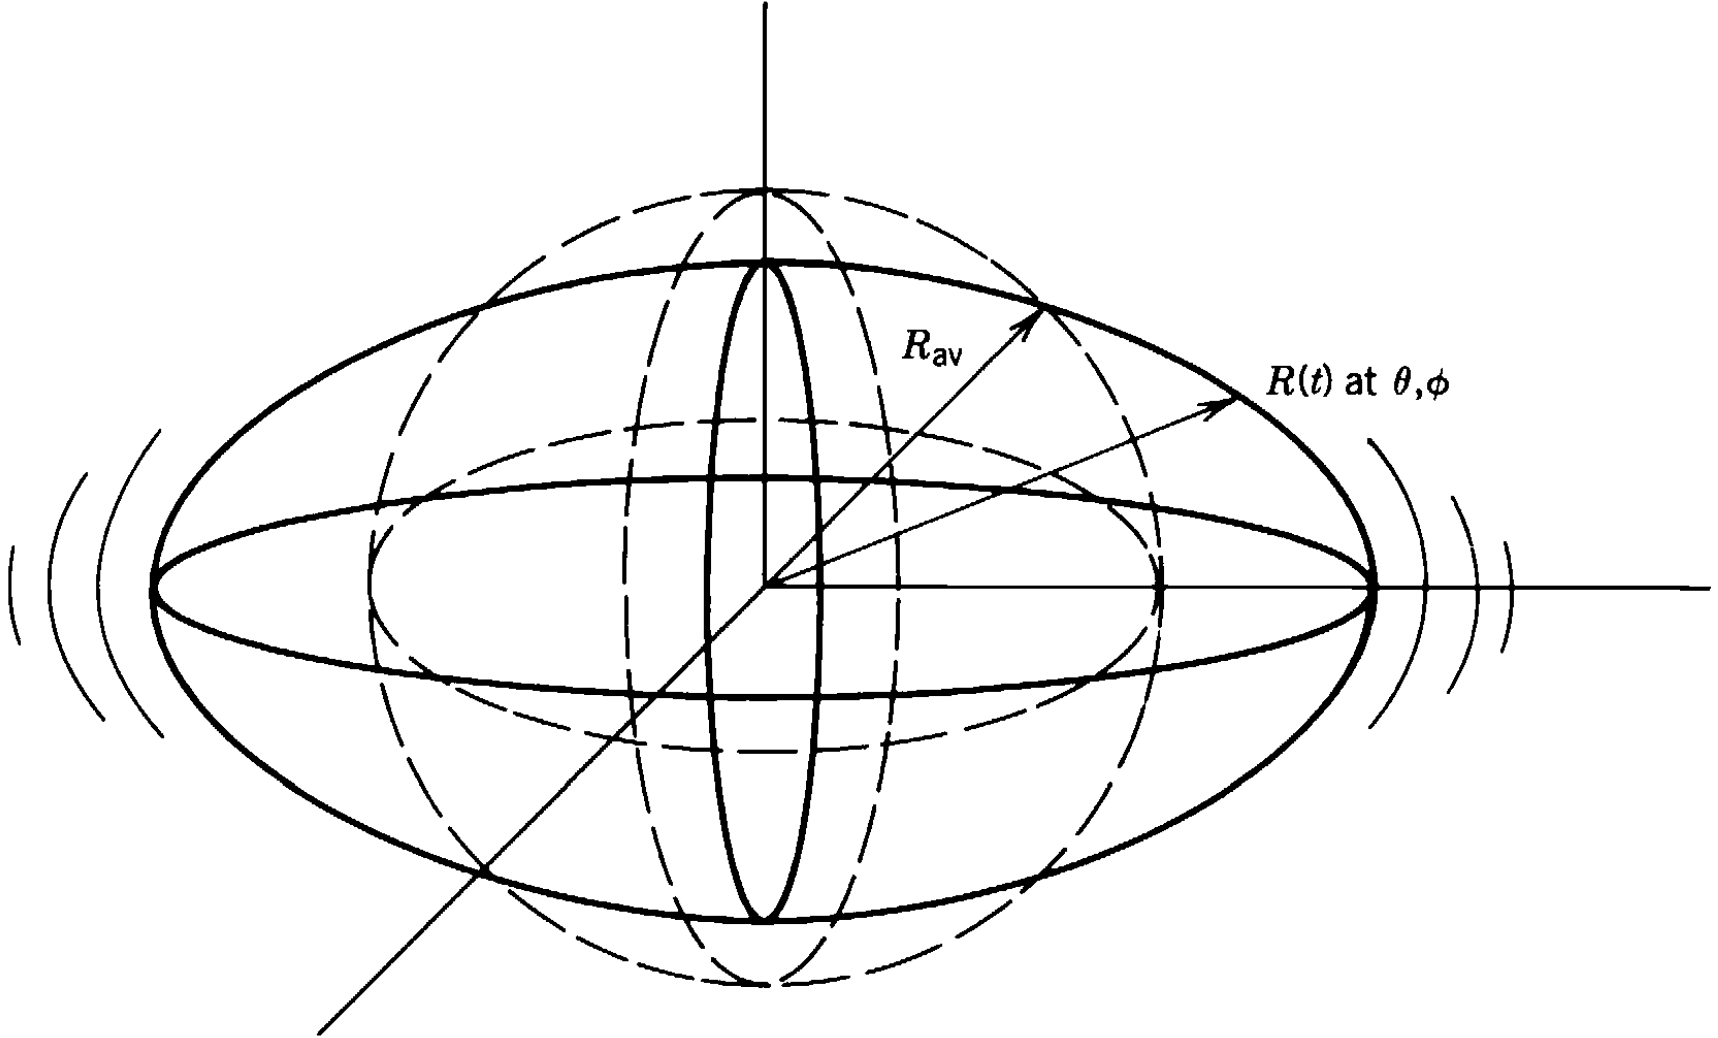
\includegraphics[width = 0.40 \textwidth]{coll-vib.png}
	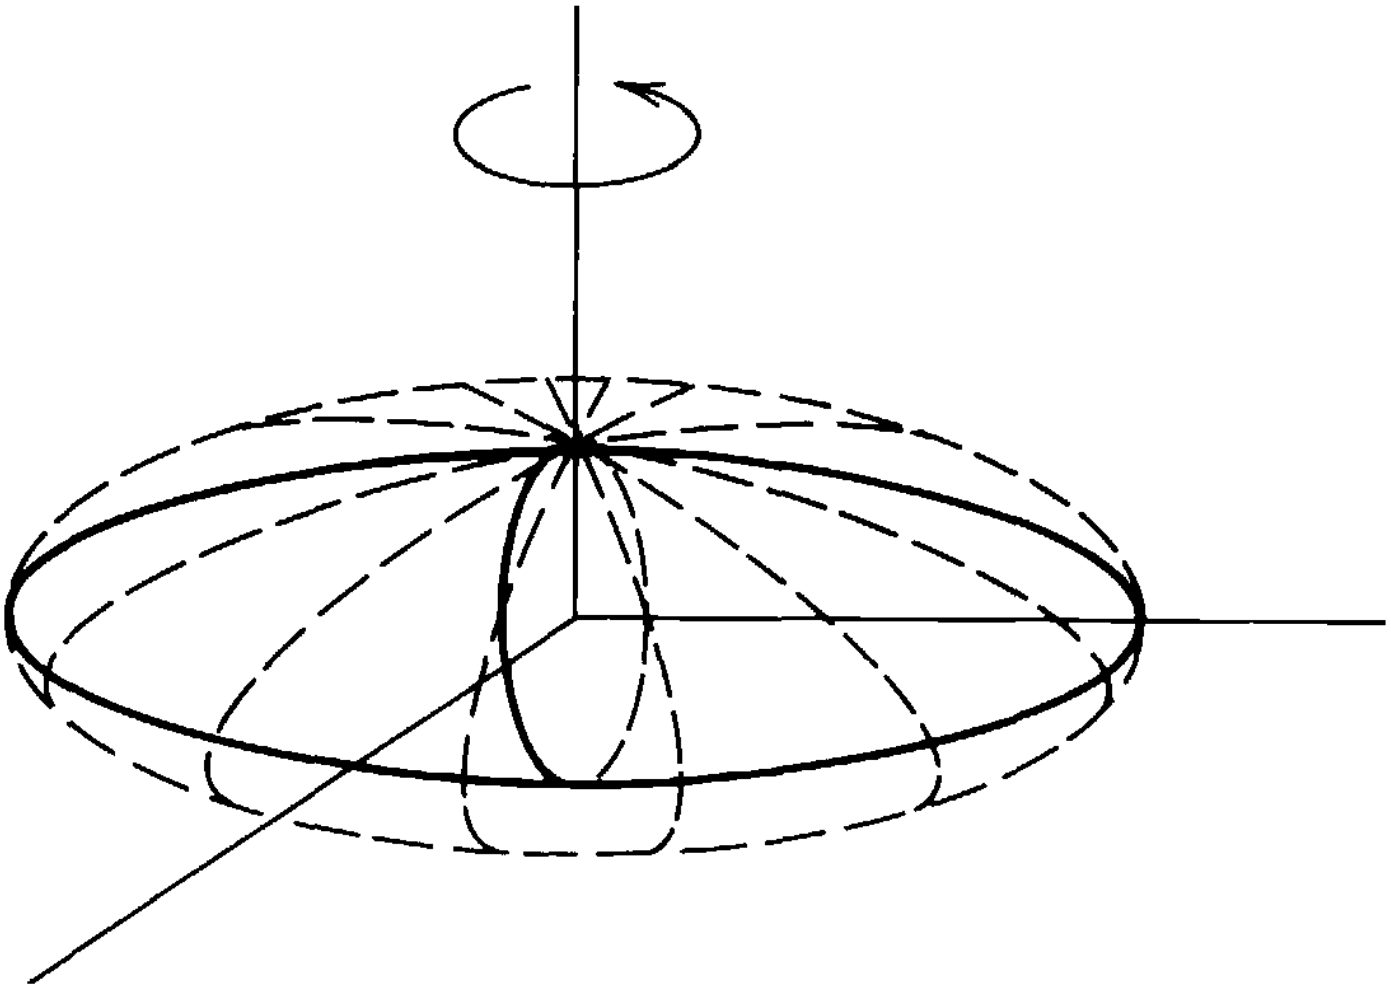
\includegraphics[width = 0.40 \textwidth]{coll-rot.png}
	\caption{Collective vibrations and rotations.}
	\label{coll}
\end{figure}

\subsection{Collective vibrations}

Sebbene la forma media del nucleo sia sferica, per $ A < 150 $, dato che esso può vibrare, la forma istantanea sarà deformata e descrivibile tramite le armoniche sferiche:
\begin{equation}
	R(\theta,\phi,t) = \braket{R} + \sum_{\lambda \ge 1} \sum_{\mu = -\lambda}^{\lambda} \alpha_{\lambda,\mu}(t) Y_{\lambda,\mu}(\theta,\phi)
	\label{eq:5.11}
\end{equation}
I coefficienti $ \alpha_{\lambda,\mu} $ non sono completamente arbitrari, ma per la simmetria di riflessione devono soddisfare $ \alpha_{\lambda,\mu} = \alpha_{\lambda,-\mu} $ (ulteriori condizioni sono imposte dall'eventuale incomprimibilità).\\
I vari termini $ \lambda $ della sommatoria trasportano un quanto di energia vibrazionale, quindi, in analogia all'elettromagnetismo, vengono detti \textit{fononi}. Ad esempio, un fonone dipolare è un quanto di energia vibrazionale con $ \lambda = 1 $ (ovvero trasporta un unità di momento angolare), un fonone quadripolare ha $ \lambda = 2 $, etc. In Fig. \ref{phon} si può vedere che un fonone dipolare causa uno spostamento del centro di massa del nucleo, dunque non può essere il risultato di forze nucleari.

\begin{figure}[!t]
	\centering
	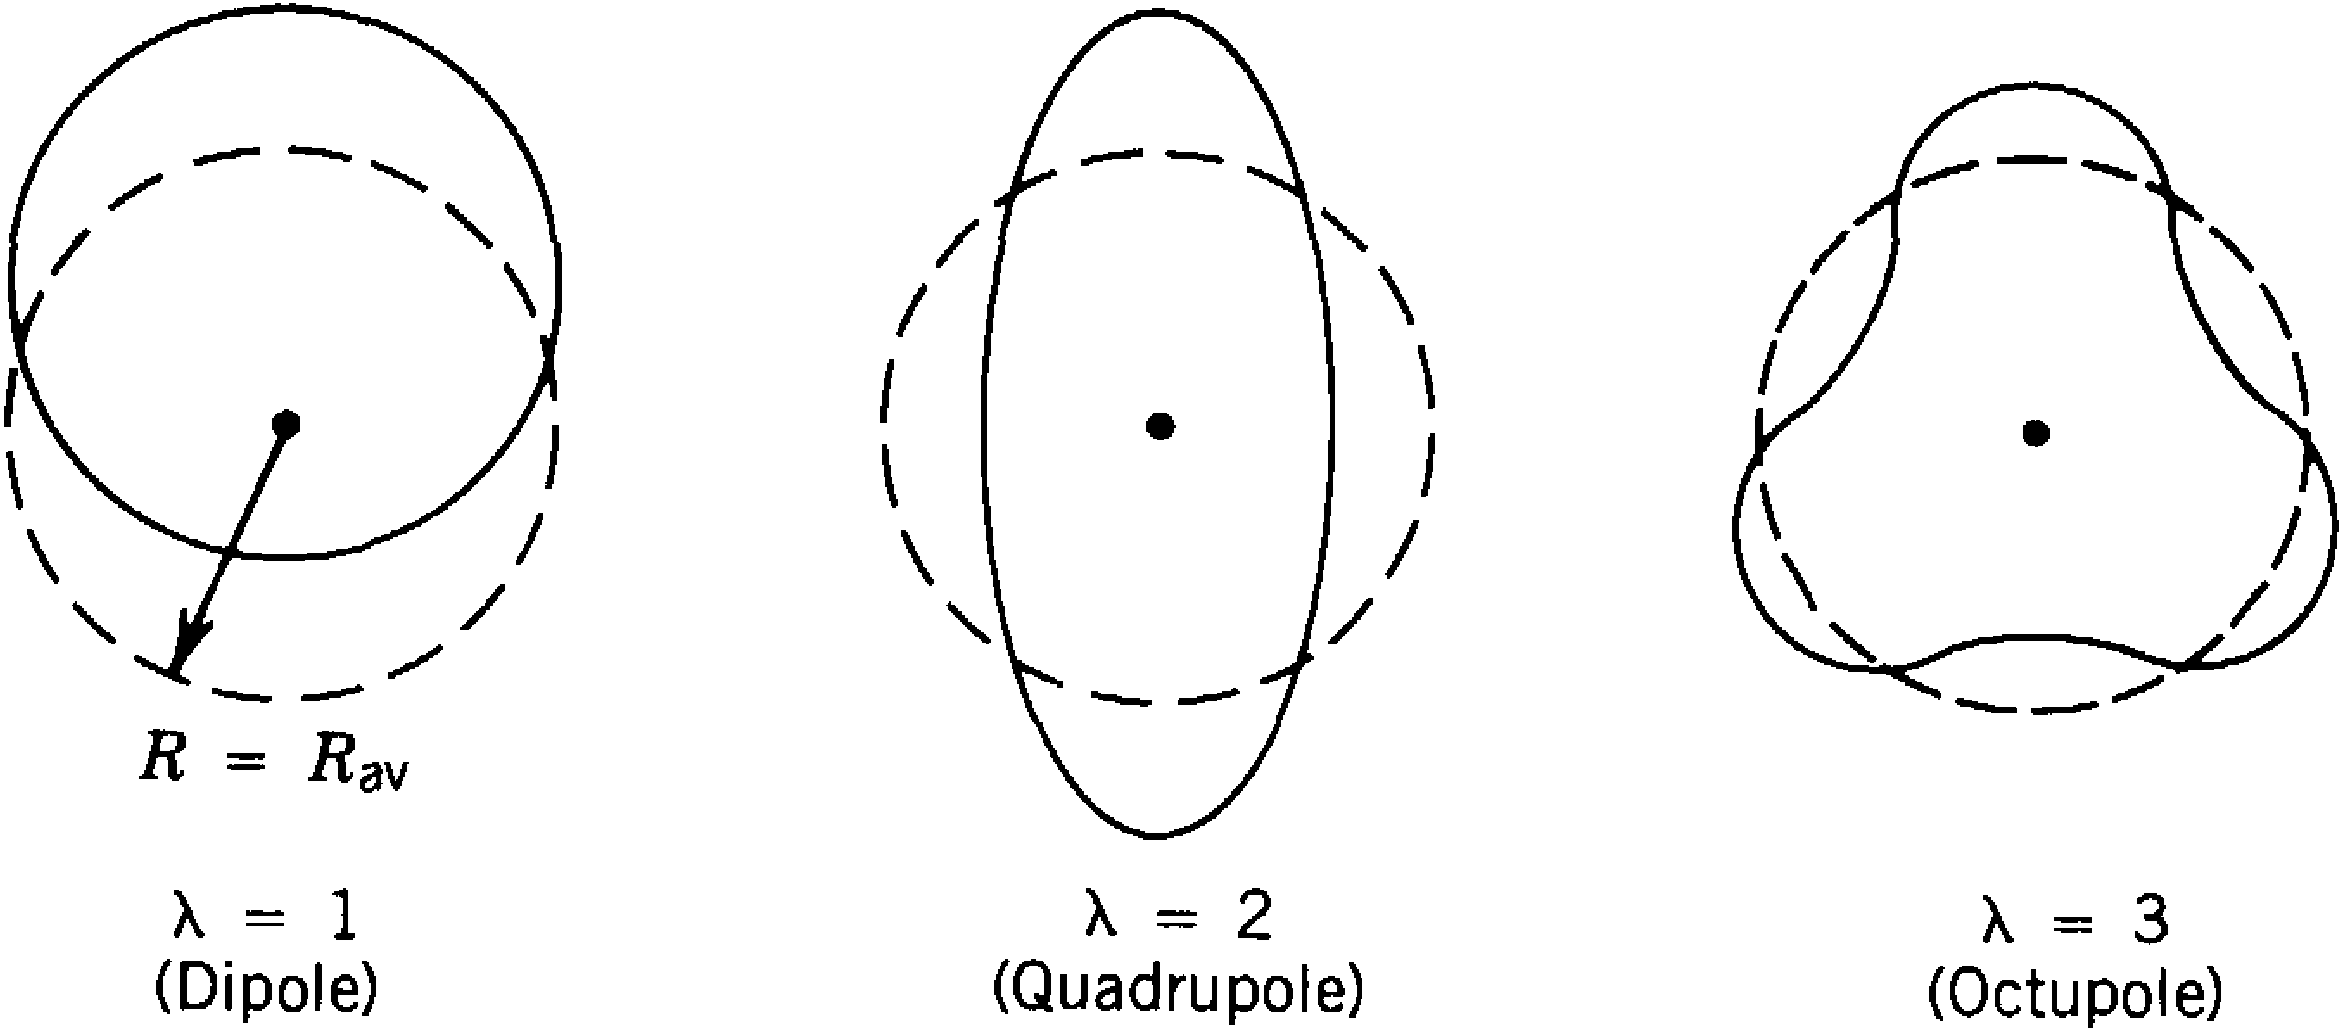
\includegraphics[width = 0.70 \textwidth]{phonons.png}
	\caption{Vibrational phonons.}
	\label{phon}
\end{figure}

Aggiungendo un fonone quadripolare ad un nucleo pari-pari nel suo ground state $ 0^+ $ il momento angolare aumenta di due unità ($ \lambda = 2 $) e la parità resta invariata ($ (-1)^{\lambda} = +1 $), dunque lo stato eccitato è $ 2^+ $: studiandone l'energia, si trova un'andamento sovrapponibile a quello in Fig. \ref{2-p} (l'energia di un fonone non è predetta, ma è un parametro regolabile). Aggiungendo un ulteriore fonone quadripolare, bisogna considerare la composizione dei momenti angolari: ciascun fonone ha 5 componenti $ \mu $, per un totale di 25 combinazioni, ma i fononi hanno funzioni d'onda totali simmetriche (poiché hanno spin intero), dunque le combinazioni si riducono a 15 e corrispondono alle componenti associate a momenti angolari $ \ell = 0,2,4 $. Ci si aspetta dunque di trovare degli stati $ 0^+ $, $ 2^+ $ e $ 4^+ $ a circa il doppio dell'energia del primo stato $ 2^+ $, e ciò e proprio quello che si osserva sperimentalmente: questi non hanno esattamente la stessa energia, confermando che anche questo modello ha le proprie semplificazioni e limitazioni, ma comunque è un'importante prova sperimentale della sua validità. In maniera analoga, si troveranno stati $ 0^+ $, $ 2^+ $, $ 3^+ $, $ 4^+ $ e $ 6^+ $ a circa il triplo dell'energia del primo $ 2^+ $, associati a tre fononi quadripolari, e così via.\\
Per quanto riguarda i fononi ottopolari, essi cambiano la parità dello stato: aggiungengo un fonone ottopolare ad un nucleo pari-pari nel ground state si ottiene uno stato eccitato $ 3^- $, con energia tipicamente superiore al tripletto associato al doppio fonone quadripolare, il quale è anche osservato nei nuclei vibrazionali, a riconferma della validità del modello.

\subsubsection{Giant resonances}
\label{sub-giant-res}

Ad energie superiori iniziano ad influire anche le eccitazioni dovute al pair breaking, dunque la trattazione si fa molto più complessa. Un fenomeno interessante, però, sono le cosiddette \textit{risonanze giganti}: queste vibrazioni avvengono ad energie estremamente elevate ($ > 10\mev $) e coinvolgono praticamente tutti i nucleoni nel nucleo.\\
Le risonanze giganti più importanti sono il monopolo gigante, in cui non c'è trasferimento di momento angolare poiché il nucleo si espande e comprime attorno alla forma sferica, decadendo poi per emissione di particelle, ed il dipolo gigante, in cui invece la distribuzione di protoni e quella di neutroni oscillano in opposizione di fase, decadendo poi per emissione di particelle e raggi $ \gamma $.\\
A livello macroscopico, le risonanze giganti possono essere descritte come le oscillazioni di una goccia attorno ad un punto d'equilibrio, mentre a livello microscopico la trattazione è estremamente difficile ma può essere fornita dal modello a shell: queste risonanze altro non sono che una sovrapposizione coerente di tutte le possibili eccitazioni particle-hole nelle varie shell nucleari, e ciò spiega le alte excitation energies.

\paragraph{Pygmy and Giant Dipole Resonance}

La risonanza vibrazionale più importante e studiata è la risonanza gigante di dipolo (GDR), nella quale tutta la distribuzione di protoni oscilla contro tutta la distribuzione dei neutroni: questo può avvenire sia a seguito dell'assorbimento di un fotone, con la componente elettrica del campo elettromagnetico che causa l'oscillazione dei protoni e lascia inalterati i neutroni, oppure a seguito di reazioni nucleari. Tipicamente si ha $ E_{\text{GDR}} \approx 80\mev \cdot A^{-1/3} $.\\
Va inoltre notato che per nuclei stabilmente deformati i tre assi d'oscillazione non sono ugugali tra loro (solo due lo sono), dunque la tipica forma approssimativamente lorentziana della GDR (vedere Fig. \ref{pgdr}) si va a deformare, fino a presentare due picchi distinti: questo è un importante indicatore di deformazioni permanenti del nuclide.\\
Oltre alla GDR, che coinvolge tutti i nucleoni, nei nuclei neutron-rich è possibile una risonanza di dipolo in cui il core, composto di protoni e neutroni, oscilla rispetto alla neutron skin: questa è detta \textit{Pygmy Dipole Resonance} (PDR), poiché avviene ad energie minori della GDR (vedere Fig. \ref{pgdr}). Si pensa che la PDR diventi estremamente preponderante man mano che si considerano nuclei sempre più esotici e neutron-rich, e ciò ha particolare rilevanza in ambito astrofisico.

\begin{figure}[!t]
	\centering
	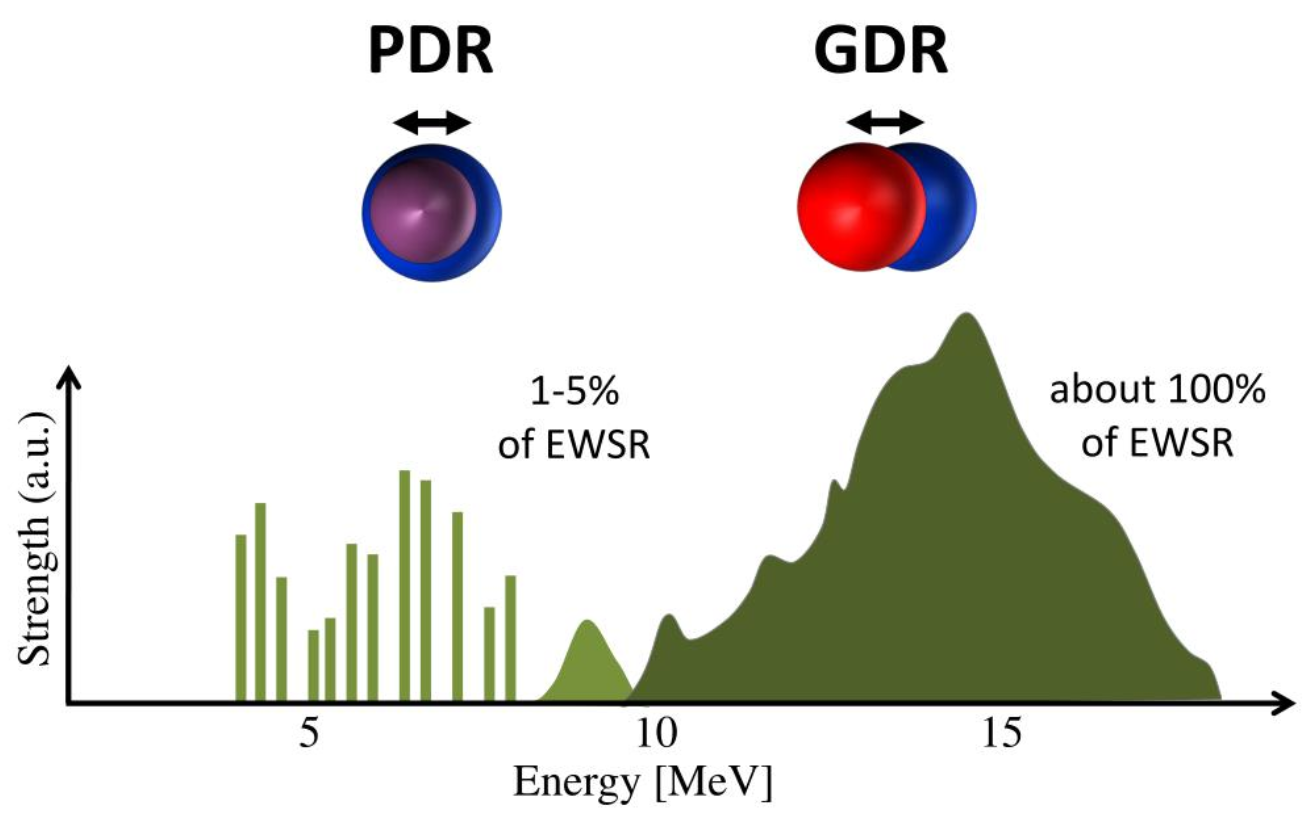
\includegraphics[width = 0.70 \textwidth]{pgdr.png}
	\caption{Pygmy and Giant Dipole Resonances and their respective probabilities.}
	\label{pgdr}
\end{figure}

\subsection{Collective rotations}

Per $ A > 150 $ la forma dei nuclei è stabilmente deformata: gran parte di questi nuclei ha parametro di deformazione (Eq. \ref{eq:5.9}) $ \beta \approx 0.30 $, dunque la differenza tra i due semiassi è circa del 30\%.\\
Dato un corpo rigido di momento d'inerzia $ \mathfrak{I} $ e momento angolare $ I $, l'energia del sistema (tratta quantisticamente) può essere espressa come:
\begin{equation}
	E(I) = \frac{I^2}{2\mathfrak{I}} = \frac{\hbar^2}{2\mathfrak{I}} I (I + 1)
	\label{eq:5.12}
\end{equation}
Nel caso di un nucleo deformato, $ I $ è un quantum number associato al momento angolare totale (sia dei protoni che dei neutroni) e lo spettro energetico così determinato corrisponde ad una serie di stati con $ I $ via via crescente, detta \textit{rotational band}: per un nucleo pari-pari il ground state è $ 0^+ $, quindi la simmetria per riflessione restringe i valori di $ I $ ai soli valori positivi, determinando la rotational band:
\begin{equation*}
	\begin{split}
		E(0^+) &= 0 \\
		E(2^+) &= 6 \frac{\hbar^2}{2\mathfrak{I}} \\
		E(4^+) &= 20 \frac{\hbar^2}{2\mathfrak{I}} \\
		E(6^+) &= 42 \frac{\hbar^2}{2\mathfrak{I}} \\
		       &\vdots
	\end{split}
\end{equation*}
Confrontando coi dati sperimentali, si trova che le energie così calcolate sono leggermente sovrastimate, suggerendo che il nucleo non si comporti propriamente come un corpo rigido. Infatti, modellando il nucleo come un corpo rigido si trova:
\begin{equation}
	\mathfrak{I}_{\text{rigid}} = \frac{2}{5} M \braket{R}^2 (1 + 0.31 \beta)
	\label{eq:5.13}
\end{equation}
Se invece lo si modella come un fluido all'interno di un contenitore ellissoidale:
\begin{equation}
	\mathfrak{I}_{\text{fluid}} = \frac{9}{8\pi} M \braket{R}^2 \beta
	\label{eq:5.14}
\end{equation}
Dai dati sperimentali, si trova che $ \mathfrak{I}_{\text{fluid}} < \mathfrak{I} < \mathfrak{I}_{\text{rigid}} $: il comportamento del nucleo è intermedio tra un corpo rigido, in cui i nucleoni sono fortemente legati tra loro, ed un fluido, in cui invece il legame nucleonico è debole (conseguenza della natura a short-range dell'interazione forte). Una possibile interpretazione per questo fatto è che non tutti i nucleoni partecipano alla rotazione, ma soltanto i nucleoni di valenza al di fuori della shell closure.\\
Va notato che per nuclei deformati è necessario modificare la forma del potenziale nucleare: esso non può più essere a simmetria sferica, ma deve avere il minimo in corrispondenza della deformazione.

\paragraph{Spettro della rotational band}

Sebbene l'energia della rotational band vari quadraticamente col momento angolare (Eq \ref{eq:5.12}), l'energia emessa dalla transizione $ \gamma $ tra due stati eccitati della rotational band varia linearmente con $ I $:
\begin{equation}
	E_{\gamma}(I) \equiv E(I + 2) - E(I) = \frac{2\hbar^2}{\mathfrak{I}} I
	\label{eq:5.15}
\end{equation}
Di conseguenza, lo spettro $ \gamma $ ottenuto con queste transizioni presenta una notevole regolarità, dato che l'energia di tali fotoni è equispaziata:
\begin{equation}
	\Delta E_{\gamma} \equiv E_{\gamma}(I + 2) - E_{\gamma}(I) = \frac{4\hbar^2}{\mathfrak{I}}
	\label{eq:5.16}
\end{equation}
Questo spettro molto regolare è caratteristico della rotational band di nuclei deformati, quindi è un ottimo indicatore per individuare tali nuclei.\\
Inoltre, misurando lo spettro energetico rotazionale, da $ \Delta E_{\gamma} $ si può ottenere una misura di $ \mathfrak{I} $ e dunque di $ \beta $, oltre ad avere una conferma teorica del rapporto costante $ E(4+) / E(2^+) \approx 3.3 $ per nuclei pesanti ($ A > 150 $).

\paragraph{Super-deformed nuclei}

Dagli studi sul momento di quadrupolo anomalo è stata scoperta l'esistenza di nuclidi che presentano delle \textit{super-deformed bands}, ovvero nuclidi con deformazioni estreme (ben oltre $ \beta \approx 0.30 $) che ruotano a velocità incredibili: il primo di questi nuclei ad essere scoperto fu il $ \ch{^{152}Dy} $ nel 1986, con una frequenza di rotazione di $ \sim 10^{21} \,\text{Hz} $. Al giorno d'oggi sono note oltre 350 super-deformed bands.










